%!TEX root = ../../dissertation.tex
%%%%%%%%%%%%%%%%%%%%%%%%%%%%%%%%%%%%%%%%%%%%%%%%%%%%%%%%%%%%%%%%%%%%%%%%%%%%%%%%
\section{Signaling Evaluation}
\label{c4:sec:evaluations}

Finally, the core network control plane load evaluations can now be tackled. The previously described dataset is thoroughly investigated several approaches to measure load and related factors are iterated.


%%%%%%%%%%%%%%%%%%%%%%%%%%%%%%%%%%%%%%%%%%%%%%%%%%%%%%%%%%%%%%%%%%%%%%%%%%%%%%%%
\subsection{Traffic Ratio Estimations}

\begin{table}
\centering
\caption{Relative device-discriminated traffic statistics extracted from the dataset.}
\label{tab:trafficstats}
	\begin{tabu}{X[1.4]X[r]X[r]X[r]X[r]X[r]}
	\toprule
	& \textbf{Flows} & \textbf{Traffic} & \textbf{Tunnels} & \textbf{\gls{gtp} pairs} & \textbf{Devices}\\ 
	\midrule
	\multicolumn{2}{c}{\textbf{By device type}}       &             &             &             &           \\
	% In TAC DB      & $99.72\%$   & $99.97\%$   & $87.57\%$   & $90.95\%$   & $80.93\%$ \\
	Smartphones      & $20.58\%$   & $12.81\%$   & $60.31\%$   & $75.99\%$   & $37.97\%$ \\
	Regular phones   & $0.26\%$    & $0.37\%$    & $5.40\%$    & $0.94\%$    & $9.25\%$  \\
	\gls{3G} dongles & $66.55\%$   & $75.12\%$   & $12.71\%$   & $9.53\%$    & $25.10\%$ \\
	\midrule
	\multicolumn{2}{c}{\textbf{By \gls{os}}}       &             &             &             &           \\
	Android          & $10.82\%$   & $6.48\%$    & $14.33\%$   & $43.33\%$   & $14.01\%$ \\
	iOS              & $7.22\%$    & $4.47\%$    & $18.91\%$   & $20.35\%$   & $7.94\%$  \\
	Symbian          & $1.02\%$    & $1.09\%$    & $21.17\%$   & $4.51\%$    & $12.97\%$ \\
	Blackberry OS    & $0.07\%$    & $0.10\%$    & $2.17\%$    & $2.60\%$    & $1.48\%$  \\
	\bottomrule
	\end{tabu}
\end{table}

To get a first grasp of the dynamics present in the dataset and the core network under investigation, Figure~\ref{tab:trafficstats} shows a small survey of the traffic composition split up by device type and \gls{os} categories. The majority of signaling messages originated from smartphones, which in turn generated only a small portion of user traffic when compared to \gls{3G} dongles.

With these numbers, the notion of active devices or tunnels can also be introduced. This only includes entities that, besides signaling, actively generated user traffic during their life cycle. Interestingly, only about \SI{82}{\percent} of all unique devices in the trace were active and could be associated with at least one traffic flow. The remaining \SI{18}{\percent} of devices still had an open \gls{gtp} tunnel but never used it. This is an extreme for the core network, as it causes a significant amount of control plane load without any actual benefit to either the network or the device. The active device distinction will also be used later on in the evaluation.

Unfortunately, the dataset does not contain any hard numbers on the volume of the signaling messages, which could be a direct indicator of the network load the control plane imposes. But using the estimation of the upper limit of a \gls{gtp} message from Section~\ref{c4:sec:gtp}, a rough upper limit on the total signaling traffic can also be derived. The following formula is used:

\begin{align}
	\phantom{,}v_s &= 2\left|S\right|(v_{gtp} + v_{udp} + v_{ip})\text{,}\\
	\phantom{.}t_r &= \frac{v_s}{v_t} \approx 0.7\si{\percent}\text{,}
\end{align}

with the signaling volume $v_s$, the set of signaling messages $S$, the estimated size of a \gls{gtp} message $v_s$, and the length of the \gls{UDP} and \gls{IP}headers. In this scenario, the traffic ratio $t_r$ of $v_s$ compared to the total traffic $v_t$ is calculated to be a minute \SI{0.7}{\percent}. Therefore, it can be safely assumed that the volume of control plane traffic appears to be a non-issue and not the bottleneck. The other load factors at the network nodes described earlier must play a more critical role, such as the memory profile of the states kept in the gateway nodes, the time required to process the large number of information held in the messages, or the imposed latency through several message round trips during transactions.

This is why the following evaluations are all intended to find some indirect approach to measure the system's load.



%%%%%%%%%%%%%%%%%%%%%%%%%%%%%%%%%%%%%%%%%%%%%%%%%%%%%%%%%%%%%%%%%%%%%%%%%%%%%%%%
\subsubsection{\texorpdfstring{\acrshort{gtp}}{GTP} Tunnel Duration}

The first indirect evaluation target will be the duration of the \gls{gtp} tunnels. This duration is directly related to the amount of occurring tunnel management signaling between the \gls{SGSN} and \gls{GGSN}. In turn, each of these signaling interactions causes processing at the two involved nodes and changes the amount of state in the form of the \gls{PDP} context. In terms of signaling messages, looking at the duration catches both tunnel create and delete messages, but no update message.

For the purpose of the evaluation the duration is defined as the interval between corresponding \gls{gtp} create and delete messages. As soon as the \gls{GGSN} sends its successful response to the create request, it can be expected that the necessary state has been created throughout the \gls{CN} and is ready to forward user packets. Similarly, after a delete message, user traffic should not be forwarded anymore. However, state may still exist and could be freed up lazily. But the latter depends entirely on the specific implementation.

As a side note, while the trace itself is only one week long, information on tunnels longer than this period can still be obtain when they were closed during the period. The trace's record on delete messages also contains the timestamp of the initial tunnel creation.

All the individual tunnel durations in the dataset are differentiated based on two factors based on the presented \gls{TAC} mechanics. The first part of the investigation looks at tunnels from different device types. After that, possible influences from the operating system are investigated. 


%%
\paragraph{Influence of the Device Type}

\begin{figure}[htb]
	\centering
	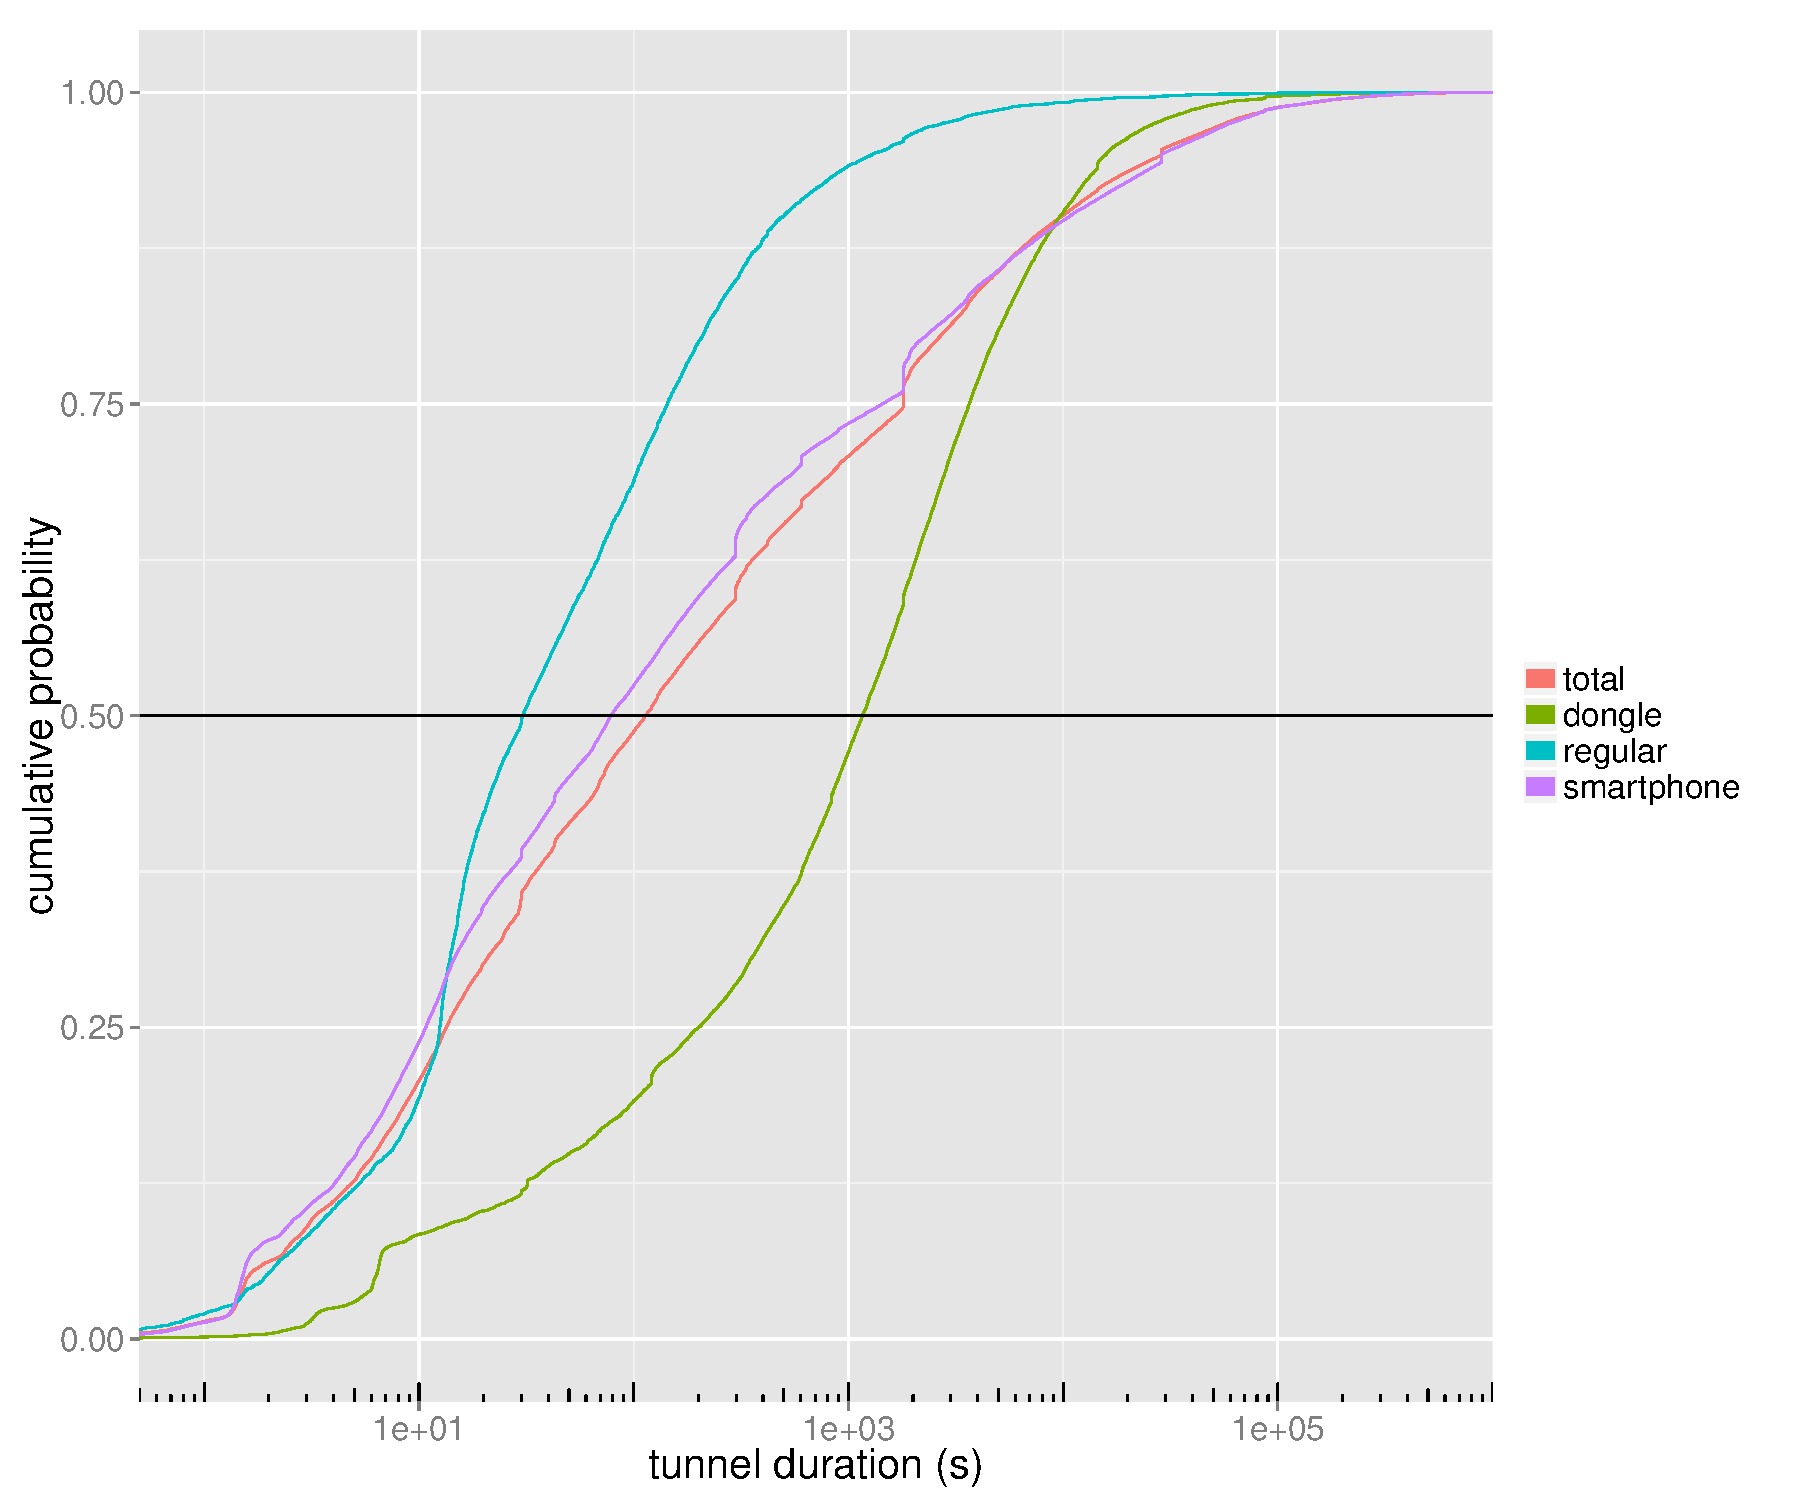
\includegraphics[width=0.9\textwidth]{images/R-tunnel-duration-device-type.pdf}
	\caption{Tunnel duration distribution, separated for \acrshort{3G} dongles, smartphones and regular phones with medians at \SI{115}{\second} (total), \SI{31}{\second} (regular), \SI{82}{\second} (smartphone), and \SI{1207}{\second} (dongle).}
\label{c4:fig:cdf-duration-device-class}
\end{figure}

Figure~\ref{c4:fig:cdf-duration-device-class} shows the \gls{ECDF} for the user tunnels and their \gls{PDP} Context durations in the dataset. In this first graph, the duration of different device classes is distinguished and put in perspective to the overall duration distribution. The devices classes here are smartphones, regular phones, and \gls{3G} dongles. It can be observed that tunnel durations range between seconds and more than one week.

The median can be clearly differentiated between device types, being much longer for \gls{3G} dongles than for mobile phones. This reflects expected user behavior very well and gives a first indicator on a possible influence of the user plane on the control plane.

Dongles are usually used with laptops to be able to work while being mobile. Dongle sessions last therefore often for extended periods longer than a few minutes up to hours. Also, this type of device is usually put into a standby mode after the period, which completely disables any mobile connections --- and therefore any associated tunnel --- instead of switching to low power radio idle modes. This is reflected in the dongle tunnel duration here as well. When compared to the other device category, dongles are more compactly centered around their median of about \SI{20}{\minute}.

A similar behavior can be observed in the regular phone distribution with values arranged tightly around the median of \SI{31}{\second}. Compared to today's smartphones, data connections on regular phones are mostly initiated explicitly by user interaction, for example through starting a browser and viewing a web page. This could also explain the comparatively low durations here.

The picture is rather different in the smartphone tunnel duration. Here, often background tasks are running over long periods of time and devices try to keep connectivity up as long as possible (while still attempting to conserve power). Overall, this could lead to the smoother distribution seen here with no clear center value.

Overall, a relatively high number of tunnels with a duration shorter than \SI{10}{\second} can also be observed. Especially the peak at about \SI{1.5}{\second} --- which is interestingly shifted to \SI{6.8}{\second} in the dongle distribution --- is of note. This is even shorter than the default values for the \gls{RRC} idle state transitions which causes the tunnel to be destroyed. It can be conjectured that these short tunnels have been explicitly removed by the \gls{UE} as no other involved state machine has timers this short.

Another distinct step at \SI{30}{\minute} in the total and smartphone distributions can be observed. As it is only present in these to categories --- and the total distribution looks to be mostly governed by smartphones --- it is reasonable to assume that the cause for this is a specific behavior observable in some aspect of smartphone related influence factors.


%%
\paragraph{Influence of the \texorpdfstring{\acrshort{os}}{OS}}

\begin{figure}[htb]
	\centering
	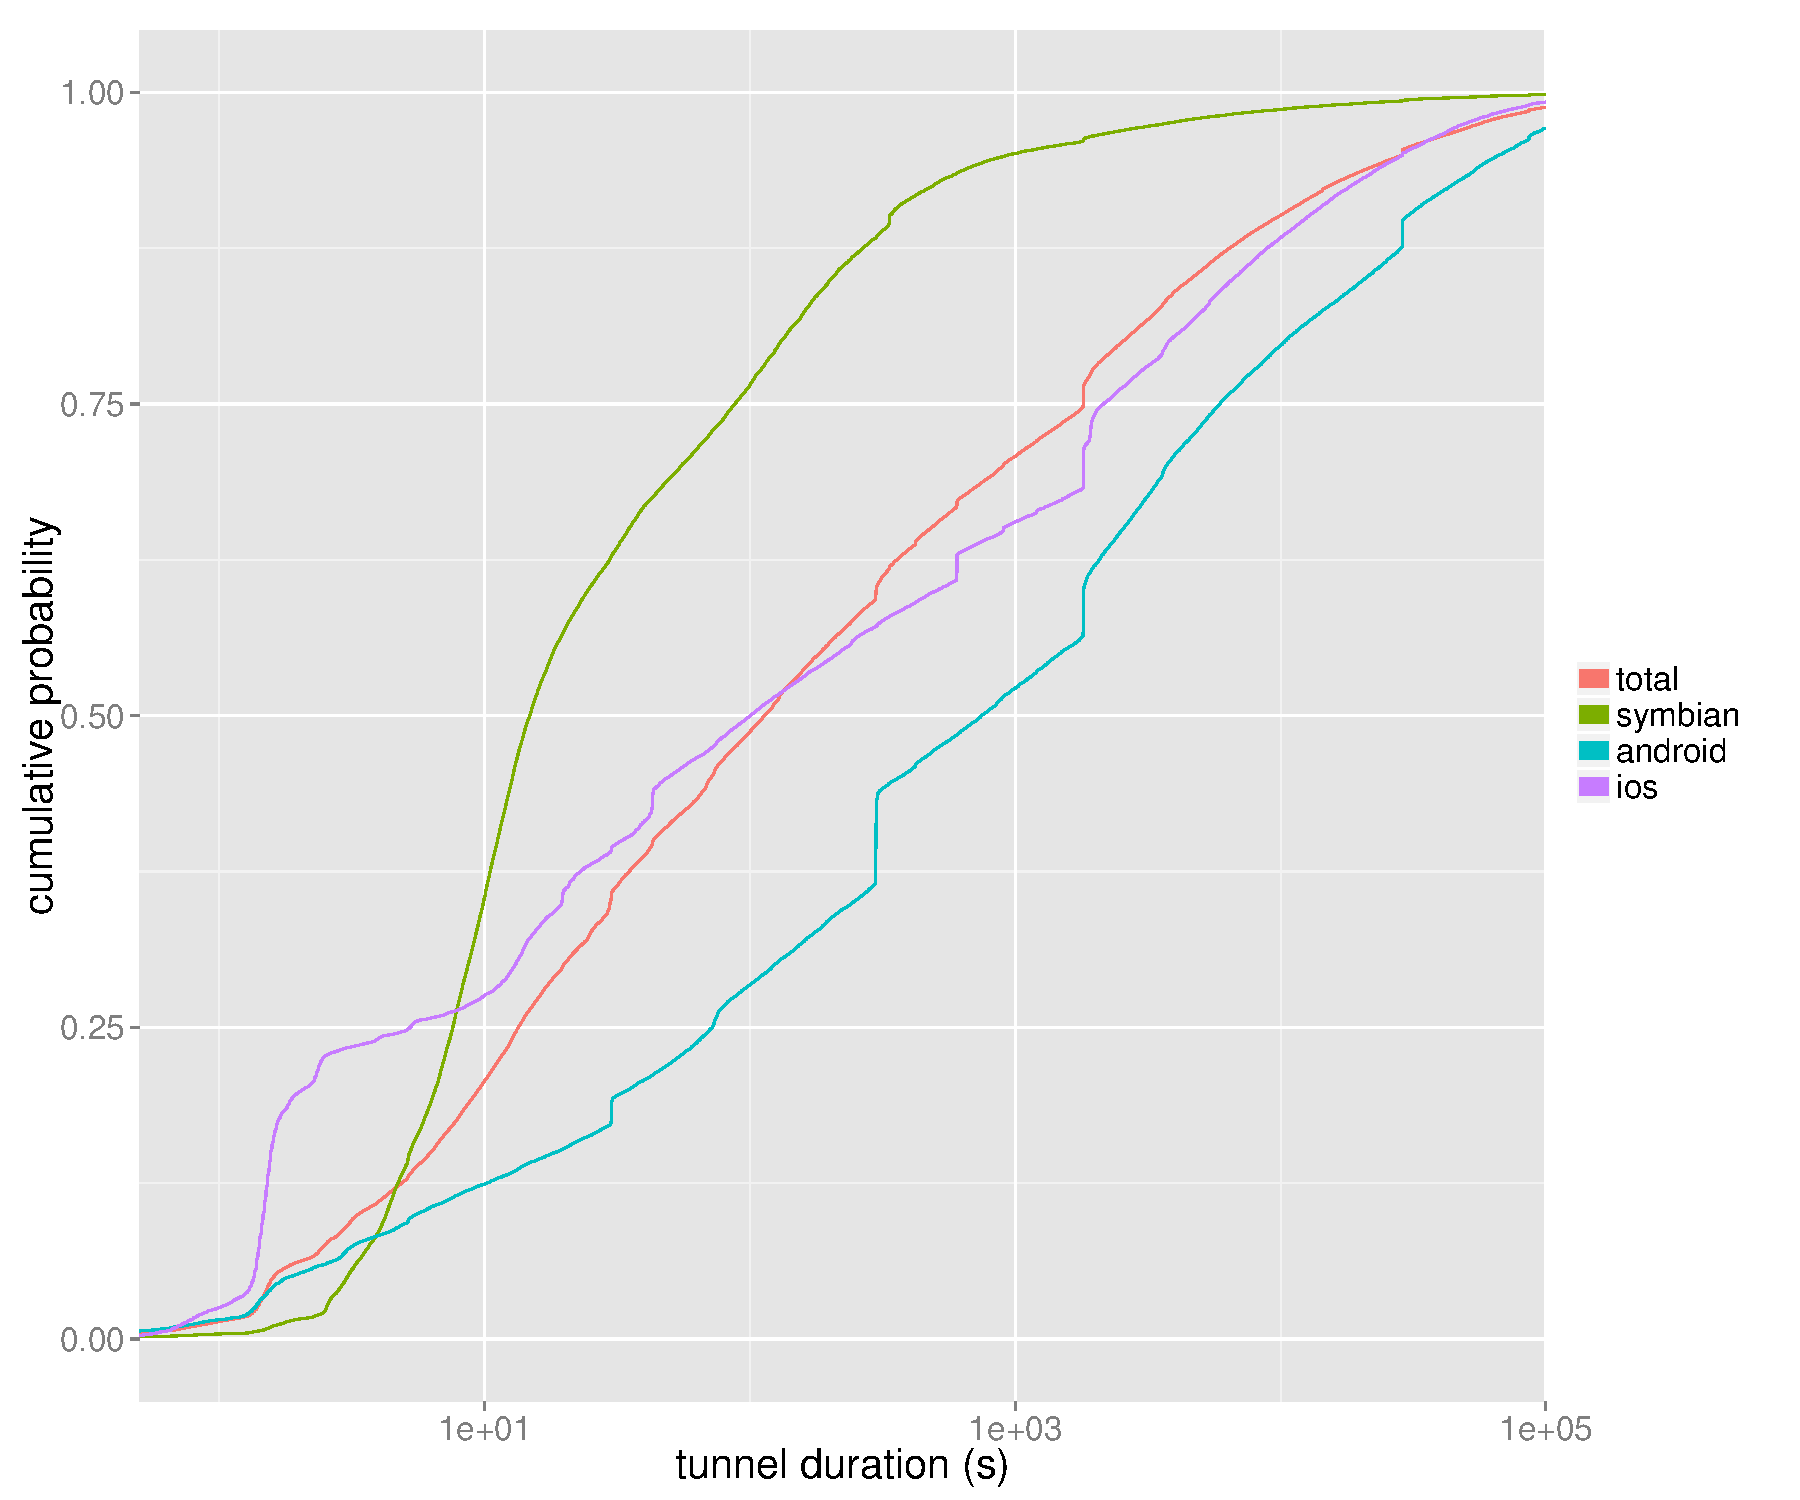
\includegraphics[width=0.9\textwidth]{images/R-tunnel-duration-operating-system.pdf}
	\caption{Tunnel duration \acrshort{CDF}, separated for select \acrshortpl{os}; Medians at \SI{115}{\second} (total), \SI{15.5}{\second} (symbian), \SI{104}{\second} (iOS), and \SI{765}{\second} (android).}
\label{c4:fig:cdf-duration-os}
\end{figure}

Next, the two phone categories are further broken down by their \gls{os}. Only the three major systems, Android, iOS, and Symbian, are identified here, the amount of other types was negligible. The smartphone category is almost exclusively represented by Android and iOS devices, while Symbian devices make up most of the regular phones but is also represented in a number of smartphone models.

Figure~\ref{c4:fig:cdf-duration-os} depicts the \gls{ECDF} of the tunnel durations of these categories in relation to the total duration distribution. They immediately exhibit a clear difference between individual \glspl{os}.

The Symbian tunnel durations are similarly distributed to the previously depicted regular phone category, albeit with an even shorter duration median of about \SI{15}{\second}. This is an indicator of the large intersection between these two groups and the explicit user traffic property attributed to regular phones.

The two smartphone-exclusive \gls{os} have remarkably similar tunnel distributions with the exception of the Android tunnel distribution shifted to much longer tunnels. This is mostly due to the larger accumulation of iOS tunnels around the previously mentioned \SI{1.5}{\second} mark. Over \SI{20}{\percent} of all tunnels established by iOS devices are shorter than \SI{2}{\second}. A possible explanation is an interaction between the described implicit background traffic happening in intervals and the efforts of iOS phones to preserve as much energy as possible. 

To this end, phones aggressively force their radio connection to the low power idle states or even completely shut off the radio immediately after transmission have ended, circumventing \gls{RRC} timers. To achieve this, iOS devices are known to implement a form of \gls{3GPP} Fast Dormancy~\cite{gsma2011fdbestpract}. It is deemed to improve device battery life, radio signaling and radio spectrum efficiency. Due the more frequent state transitions it also could cause an increase in core network tunnel management signaling, which is probably what happened in the iOS case depicted in the \gls{ECDF}.

Another set of tunnel duration accumulations are also visible in the \gls{os} distributions. Two types of steps should be distinguished here. First are accumulations that occur across multiple or all categories. This points to an influence source outside of the specific category. If the artifact is present in every distribution it is even likely, that the source is a behavior of the network's state machines. The second type of accumulation is local to one or some categories, which places the root cause into the region of these categories and their related influence factors. 

In case of the \gls{os} category, additionally, peaks at \SI{30}{\second}, \SI{300}{\second}, and \SI{600}{\second} can be observed. However, whether this behavior can be attributed directly to the operating systems themselves cannot be decided just by looking at these distribution. Other factors, e.g., the device's baseband and user traffic dynamics, also play a role. 


%%
\paragraph{Influence of the Time of Day}

\begin{figure}[htb]
	\centering
	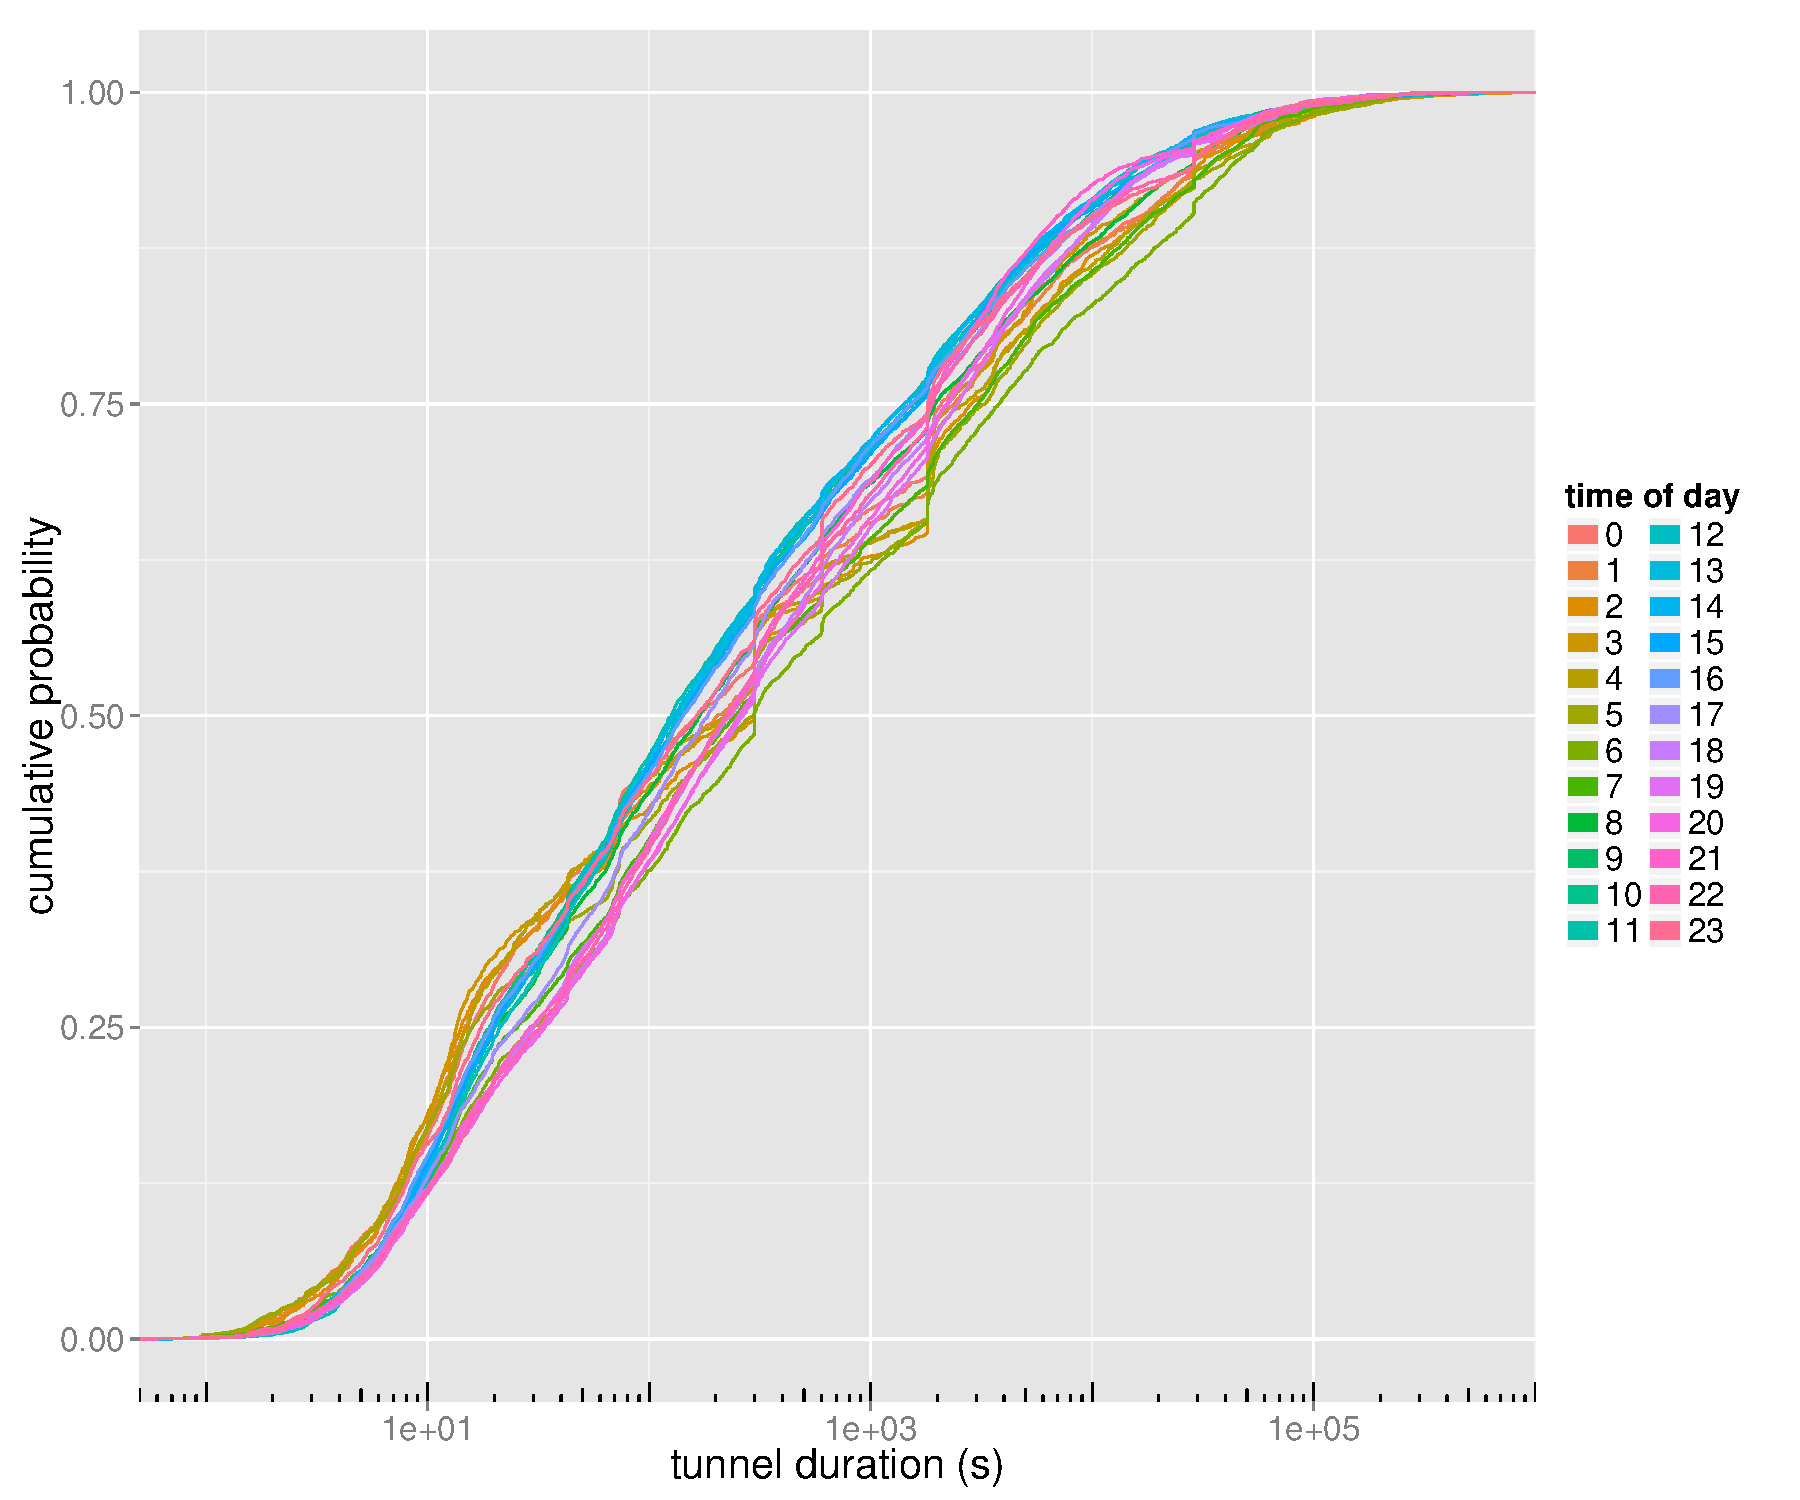
\includegraphics[width=0.9\textwidth]{images/R-duration-timeofday-ecdf.pdf}
	\caption{Tunnel duration of all active tunnels by time of day.}
\label{c4:fig:duration-timeofday-ecdf}
\end{figure}

In addition to device factors, diurnal effects could also play a role in the duration of tunnels. Figure~\ref{c4:fig:duration-timeofday-ecdf} depicts $24$ individual \glspl{ECDF} of the tunnel duration for each hour of a day. While no clear distinctions are visible, there is a trendto shorter tunnels in the early morning hours. The early afternoon hours tend to produce tunnels more centered around the middle duration range. Even longer tunnels should be treated with reservation, as they exceed the length of their assigned time slot in the \gls{ECDF} and span a larger time frame. Only the tunnel creation point is guaranteed to be in the slot.


%%
\paragraph{Influence of Other Factors}

Due to the nature of the trace dataset at hand many other influence factors are hard or outright impossible to distinguish. Some factors are unknown from the \gls{CN} perspective, as the mentioned device baseband, while others have not been recorded in the trace.

For example, it would theoretically be possible to investigate the influence of the \gls{RAT} as it is an \gls{IE} in the \gls{gtp} messages and also recorded in the trace. The radio access parts of \gls{GSM} and \gls{UMTS} are completely different --- including the \gls{RRC} state machines which were depicted in Figure~\ref{c4:fig:mmstatemodel} --- and therefore could also differ in their control plane load impact on the core. However, the \gls{RAT} \gls{IE} is optional and only set in less than \SI{1}{\percent} of the available records. As the radio access can change even during an existing tunnel --- in which case the \gls{GGSN} receives a \gls{gtp} update request informing the node about the change --- a complete picture without gaps would be required to do any investigation on this.


%%
\paragraph{Influence Strength of the Categories}

\begin{figure}[htb]
	\centering
	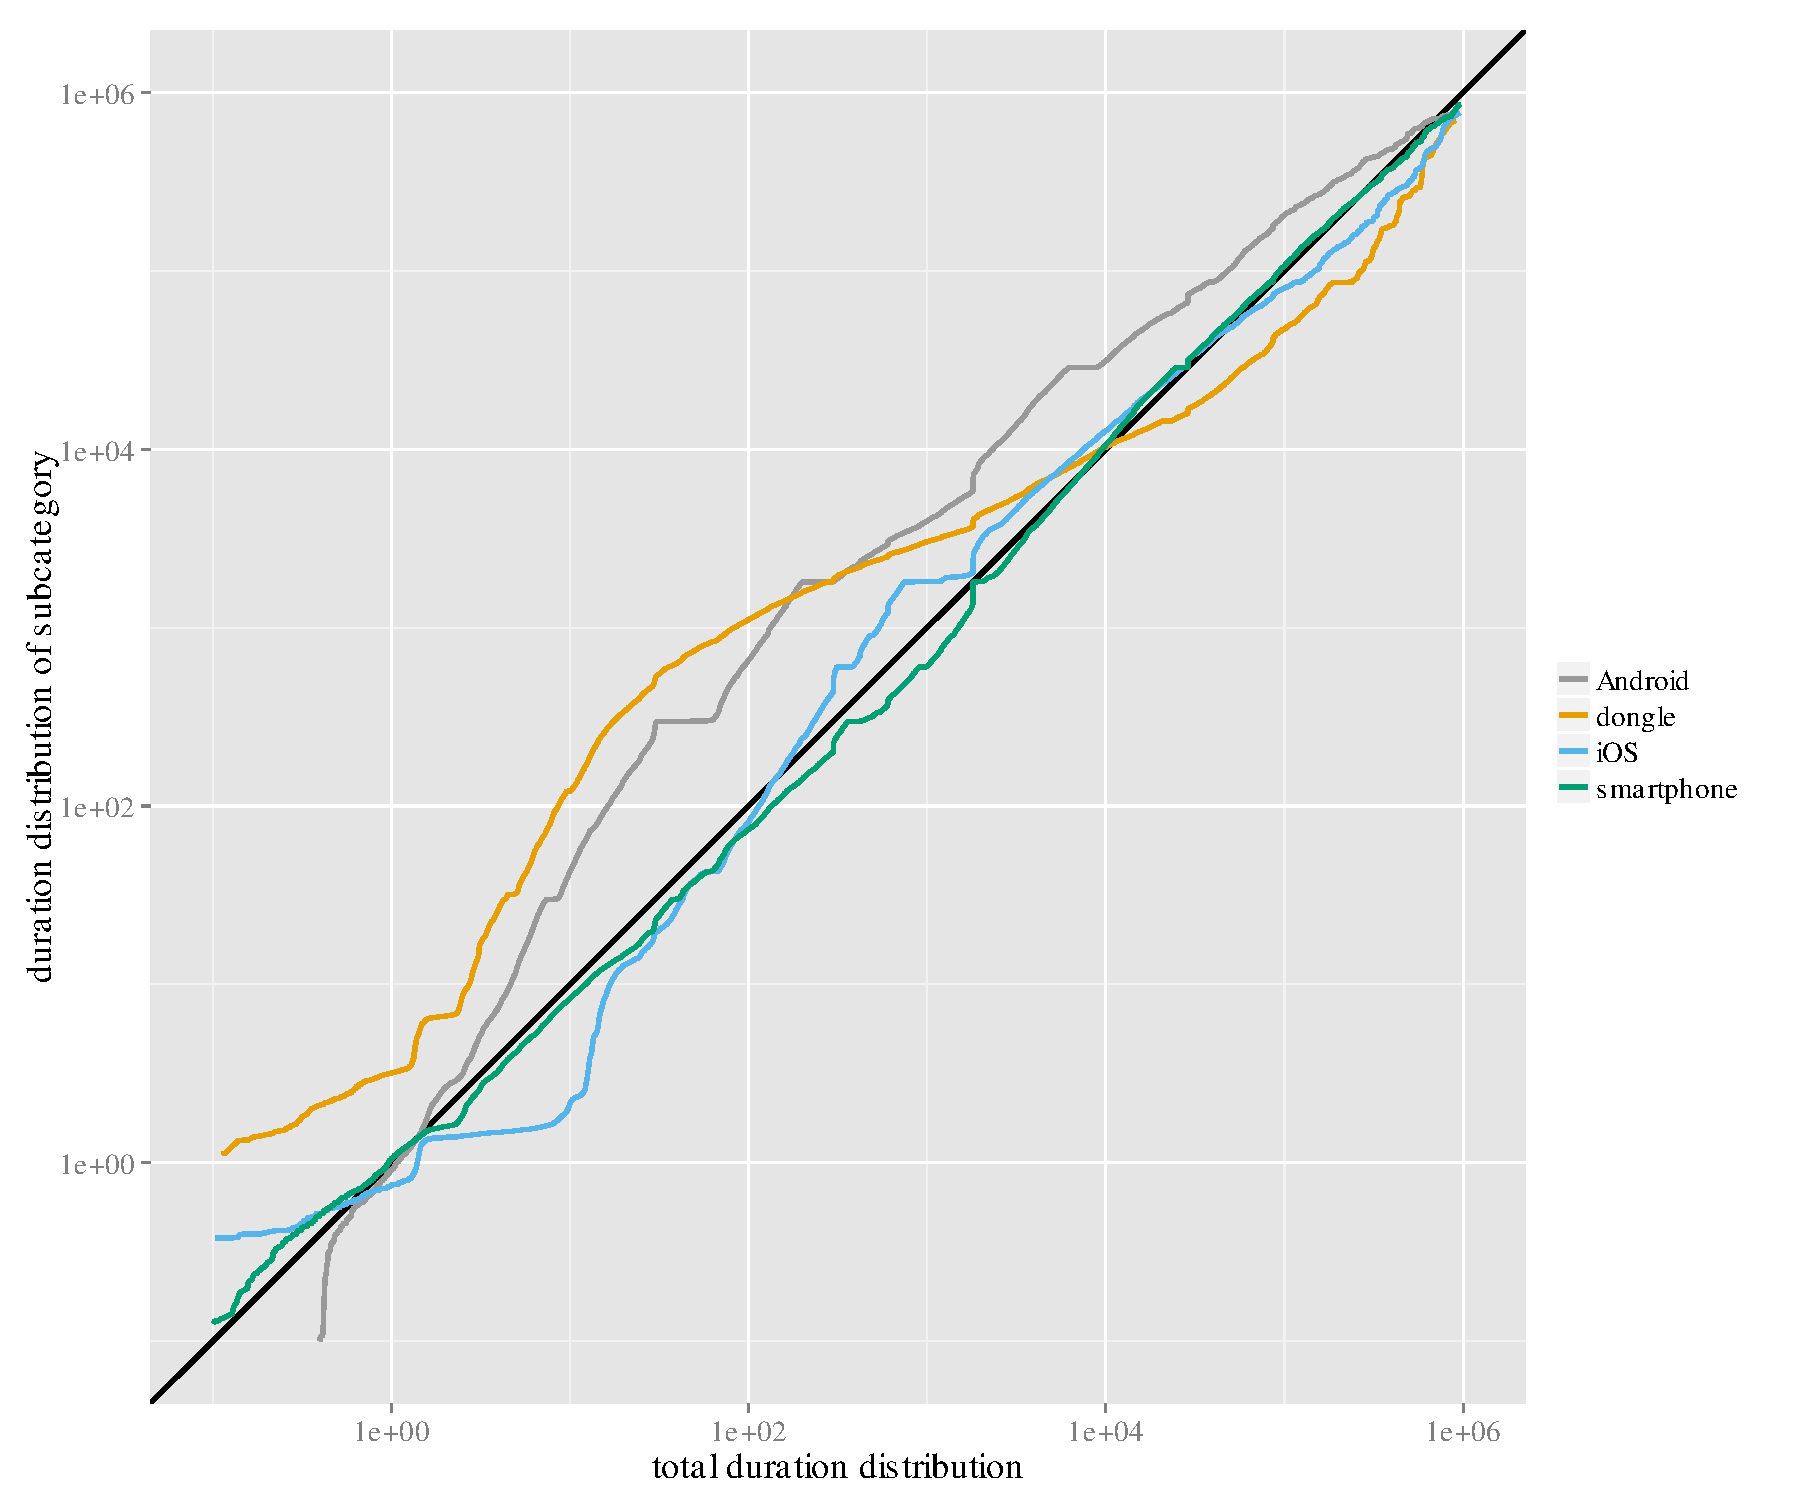
\includegraphics[width=0.9\textwidth]{images/R-duration-qq-category-comparison.pdf}
	\caption{Q-Q Plots of the tunnel duration distributions in comparison to device classification categories.}
\label{c4:fig:qq-plots}
\end{figure}


To ascertain which of the investigated device categories influences the total duration distribution most, Q-Q plots are created and investigated. It is conjectured, that the amount of influence on the duration distribution is correlated to the influence on the control plane load. In theory, if both durations follow the same distribution, one expects a straight diagonal $y=x$ line through the origin. A steeper incline indicates more compact regions in the distribution plotted on the $x$ axis and vice versa.

The Q-Q plots in Figure~\ref{c4:fig:qq-plots} compare the total tunnel duration distribution to the duration distribution of the dongle, smartphone, Android, and iOS classification cateogries. It can be observed, that the smartphone duration distribution is distributed almost equally to the total except for minor variations. However, the \gls{3G} dongle tunnel durations follow a very different distribution. Their effect on the total duration distribution seems to be negligible despite the  large amount of traffic they are causing. This is also a first indicator, that smartphones might have a larger impact on signaling than other device types.

Looking closer at the smartphone category, Q-Q plots of the two major \glspl{os} are investigated. With the exception of the large below \SI{2}{\second} peak in the lower tail of the distribution, iOS device tunnel durations are very similar to the overall tunnel duration distribution. The same can not be said about the Android distribution, which deviates somewhat in the distribution's center but is similar to the total distribution in the upper tail. Even devices with just a different \glspl{os} seem to strongly differ in their influence on duration distribution and therefore on signaling.

\begin{figure}[htb]
	\centering
	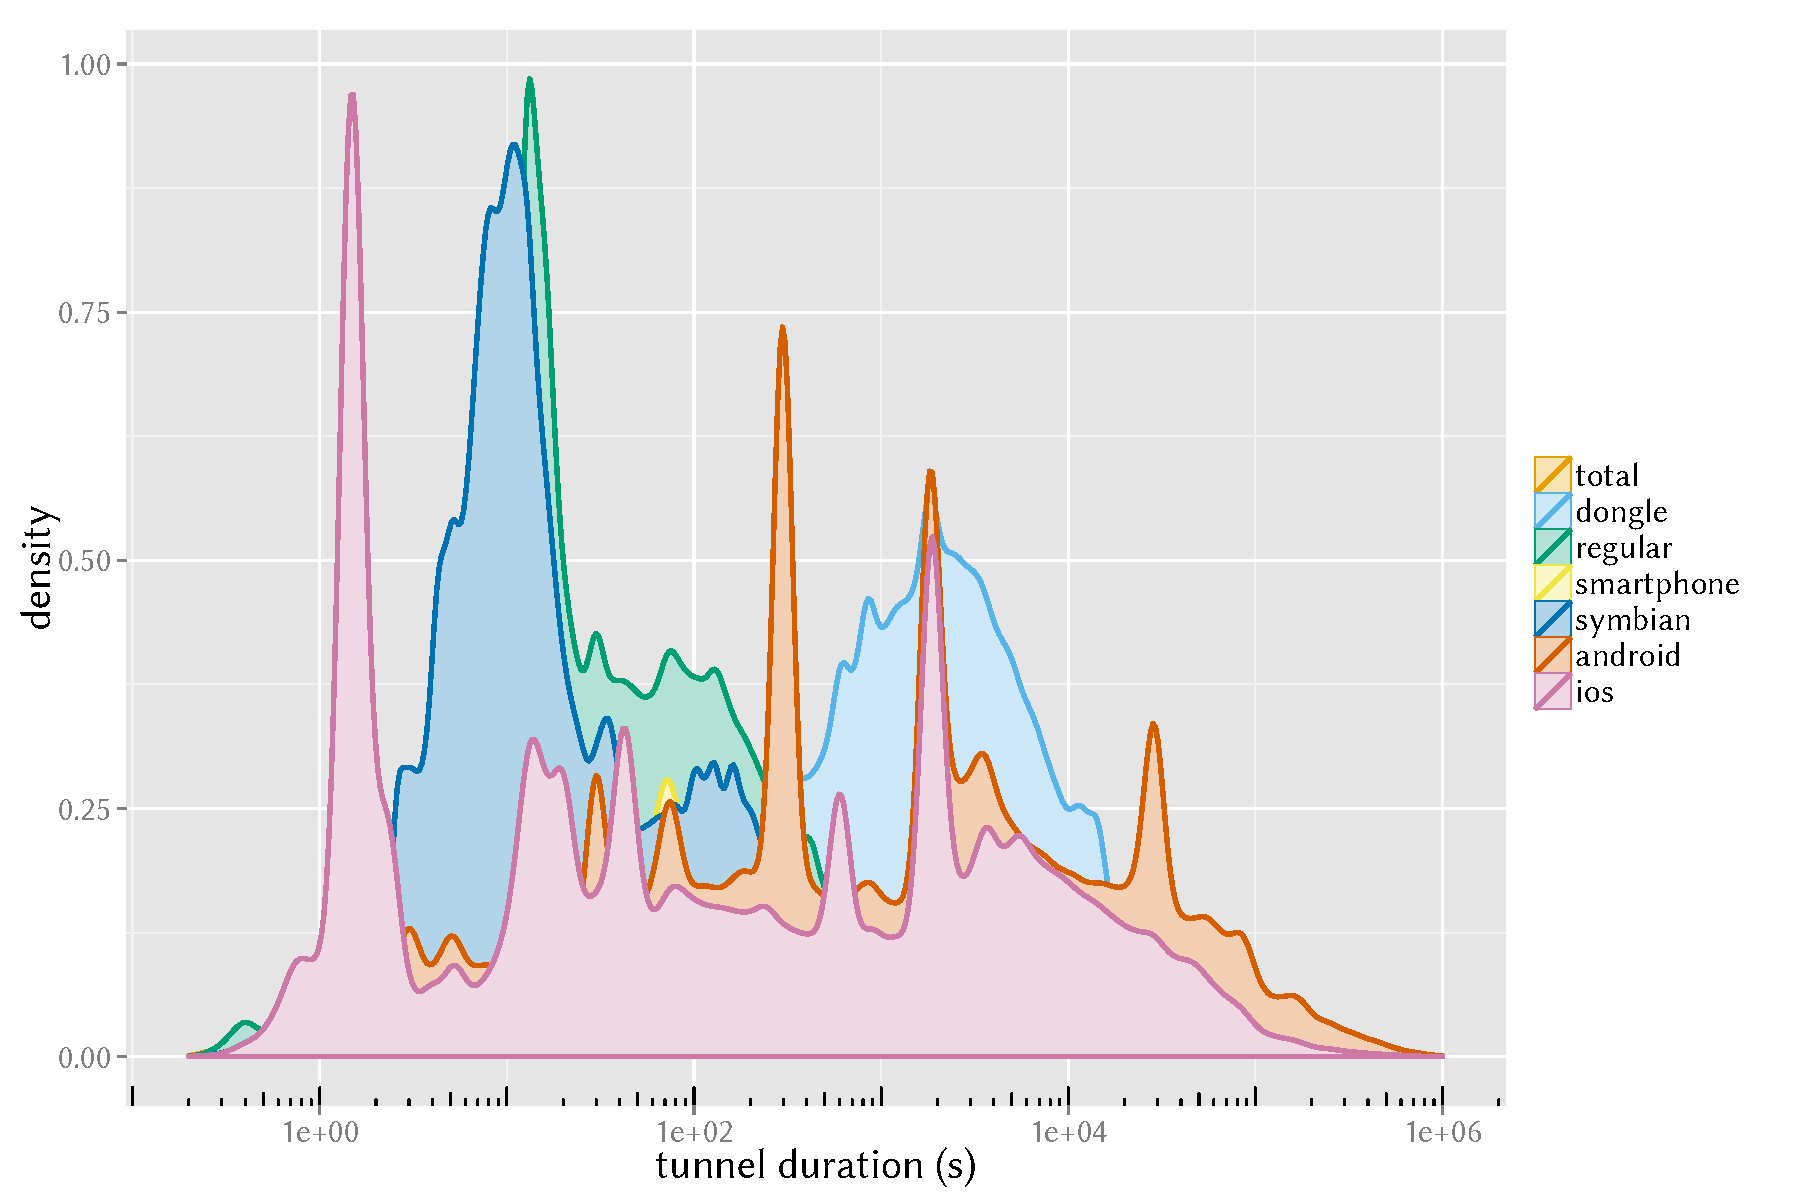
\includegraphics[width=0.9\textwidth]{images/R-duration-classification-density.pdf}
	\caption{Logscale density plot of the tunnel duration with all classifications.}
\label{c4:fig:durations-density}
\end{figure}


Figure~\ref{c4:fig:durations-density} attempts to depict where in their distributions the investigated device categories show the most impact on the total distribution. The plot shows the density of all previously investigated device influence categories.

It is evident that the durations are not evenly distributed, but rather follow sharp spikes. One of largest spike across all categories is the one at a duration of \SI{30}{\minute}, with about \SI{1.8}{\percent} of all tunnels in the network falling into that region. Since this spike happens across all device types, it makes a rather strong case for being induced by the network. On the other hand, the bulk of tunnel durations in the short-to-medium range does not seem to be governed by the two major smartphone operation systems but by other devices in the network, which do not show major spikes in other bins.

Besides the long-tailed behavior in the upper tail of the tunnel durations another slight accumulation effect, repeating itself every \SIrange{6}{7}{\day}, is present in the upper tail. This phenomenon is as yet of unknown origin and does not coincide with any known timers of the \gls{3G} mobile network.

The investigation of this data leads to the conclusion that the planning and dimensioning of the control plane needs to watch the behavior of smartphones more carefully than that device types.


%%%%%%%%%%%%%%%%%%%%%%%%%%%%%%%%%%%%%%%%%%%%%%%%%%%%%%%%%%%%%%%%%%%%%%%%%%%%%%%
\subsubsection{\texorpdfstring{\acrshort{gtp}}{GTP} Tunnel Arrivals}

The duration of \gls{gtp} tunnels is but one aspect of influence on control plane load. The arrival process of these tunnels is also interesting in itself. Specifically, this mean the arrival of tunnel requests, i.e.\gls{gtp} create requests, at the \gls{GGSN}. 

An arrival process can be described in two distinct ways. First by the number of arrivals in a given time interval. Second, by the \gls{IAT}, the time between two consecutive tunnel arrivals. Depending on the choice one has to deal with either a discrete or a continuous distribution.

Here, the tunnel arrival process is investigated with both approaches. This also adds to the foundation of the load model constructed in the next chapter. Note, that the notion of classifying arrivals into influence categories based on device specifics is omitted here. An investigation of this process can not be realistically be conducted categorized and still relate to the total system load.

\begin{figure}[htb]
	\centering
	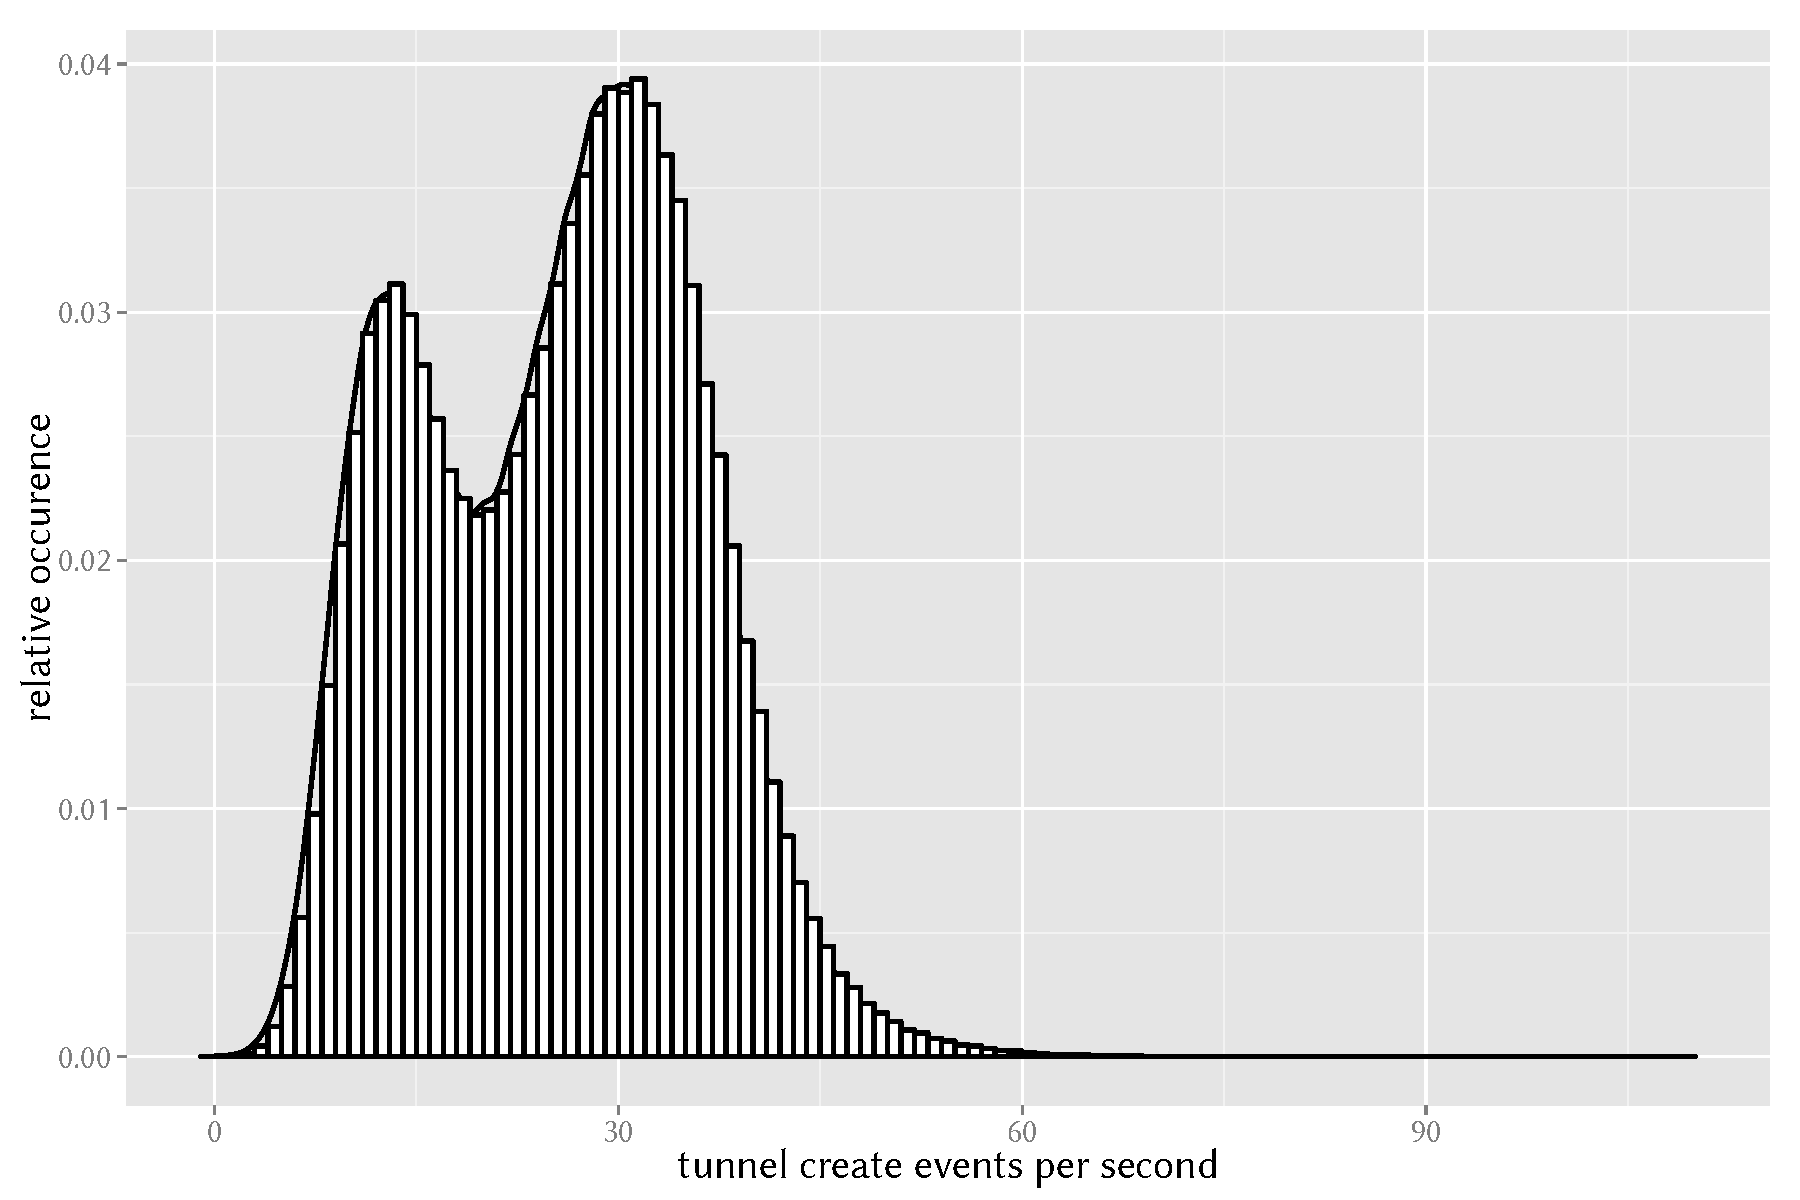
\includegraphics[width=0.9\textwidth]{images/R-create-frequency.pdf}
	\caption{Tunnel arrivals histogram overlaid with a density plot.}
\label{c4:fig:freq-arrivals}
\end{figure}

Figure~\ref{c4:fig:freq-arrivals} depicts a histogram the number of tunnel arrivals per second during the whole trace duration period. Of note is the clear bimodal nature with one peak around twelve and the other in the low thirties. While the distribution is rather compact around these two peaks, there are some clear outliers peaking at $107$ arrivals per second. If the hypothesis of the correlation between signaling load and number of arrivals holds, it can be assumed that load is not constant but rather switches between two modes with some periods of very high load induced by an increased number of arrivals.

\begin{figure}[htb]
	\centering
	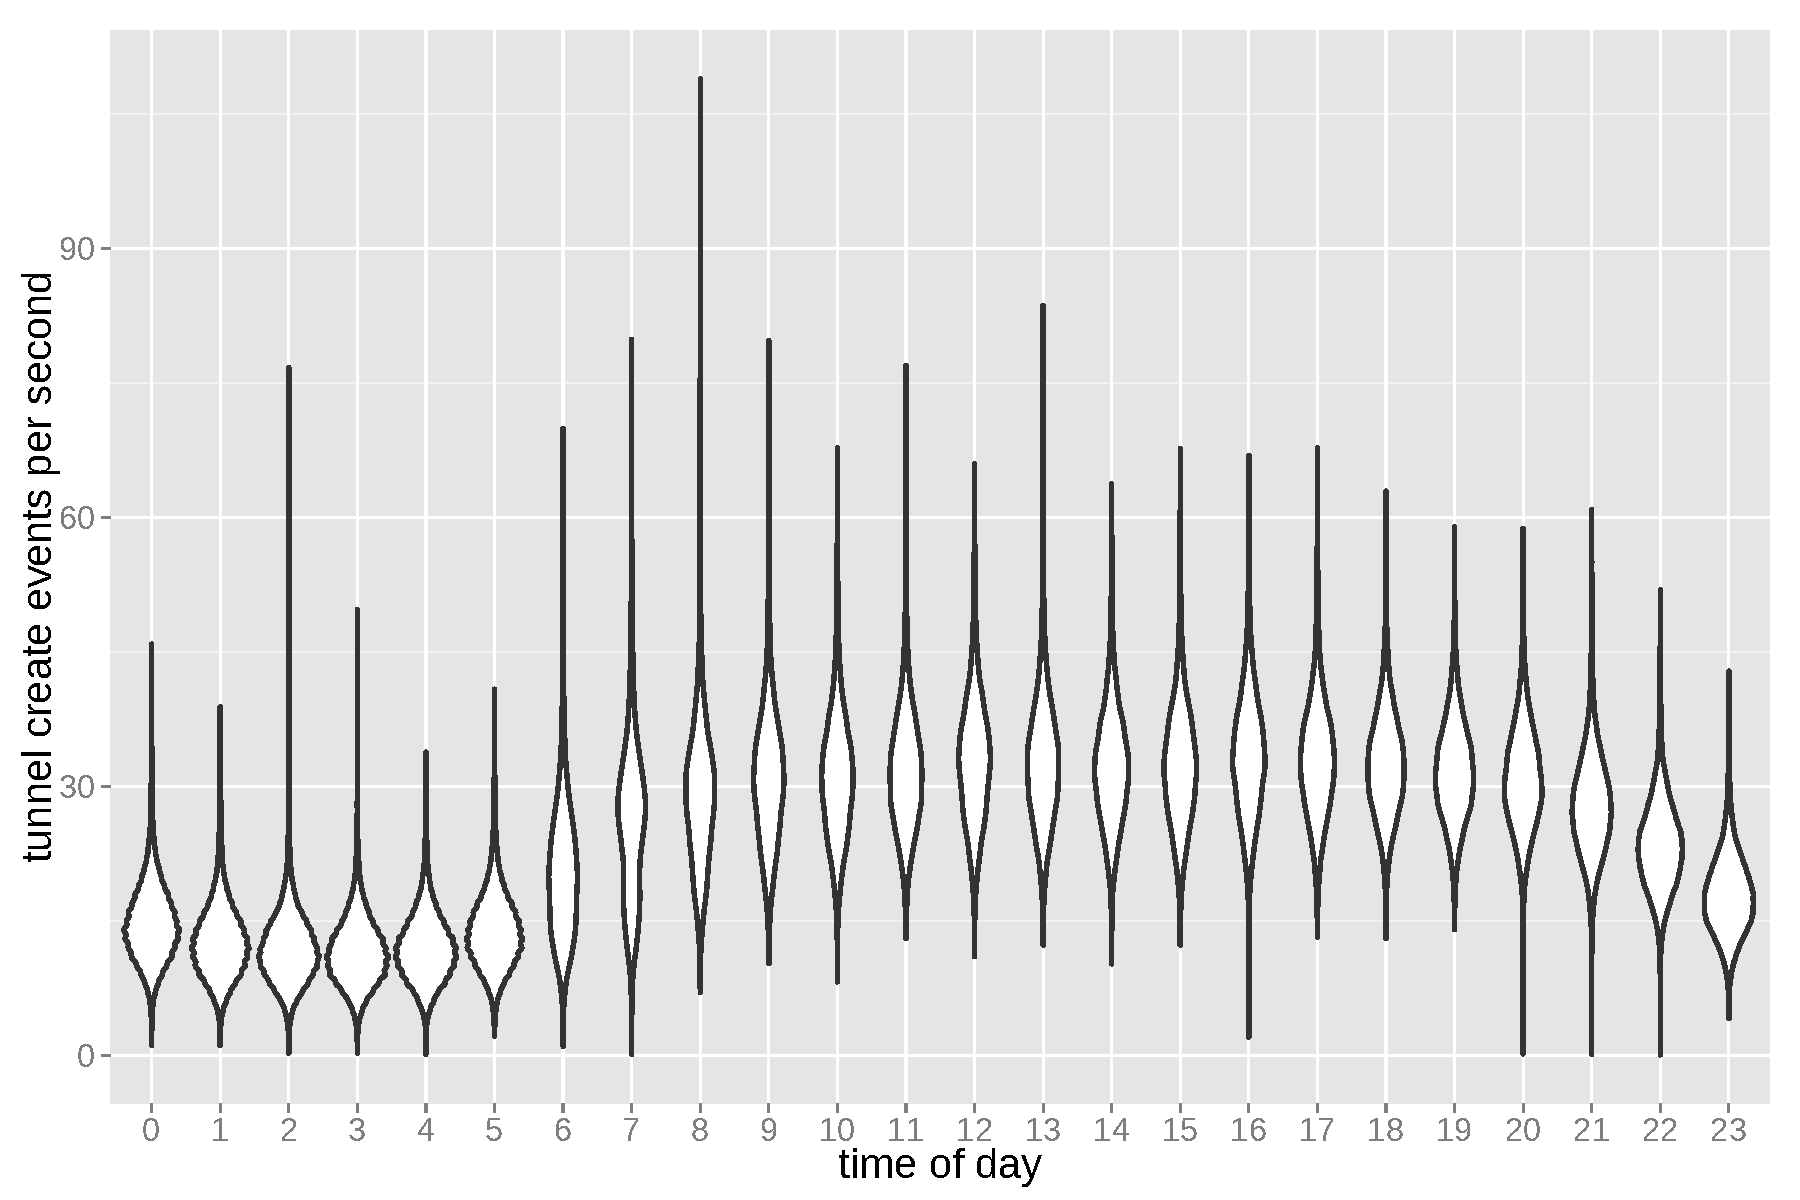
\includegraphics[width=0.9\textwidth]{images/R-createspersecond-1h-violin.pdf}
	\caption{Violin plot of tunnel arrivals in one second per time of day.}
\label{c4:fig:freq-arrivals-per-second-violin}
\end{figure}

A reasonable cause for the occurrence of these two modes can be found in the diurnal arrival patterns. Figure~\ref{c4:fig:freq-arrivals-per-second-violin} contains a violin plot of the tunnel arrivals. This type of plot is similar to a box plot but additionally shows the density of the individual items on the vertical axis. Here the arrivals are broken down to hourly slots. 

The nocturnal plateau of arrivals between midnight and \formattime{5}{0}{0} and the longer daytime plateau between \formattime{8}{0}{0} and \formattime{19}{0}{0} match the two modes found in the histogram. In between are short transition phases. The density of the arrivals during daytime indicates a spread of the number of arrivals over a larger range. This could be an indication of load fluctuations in the system.

\begin{figure}[htb]
	\centering
	\begin{subfigure}[b]{0.5\textwidth}    
		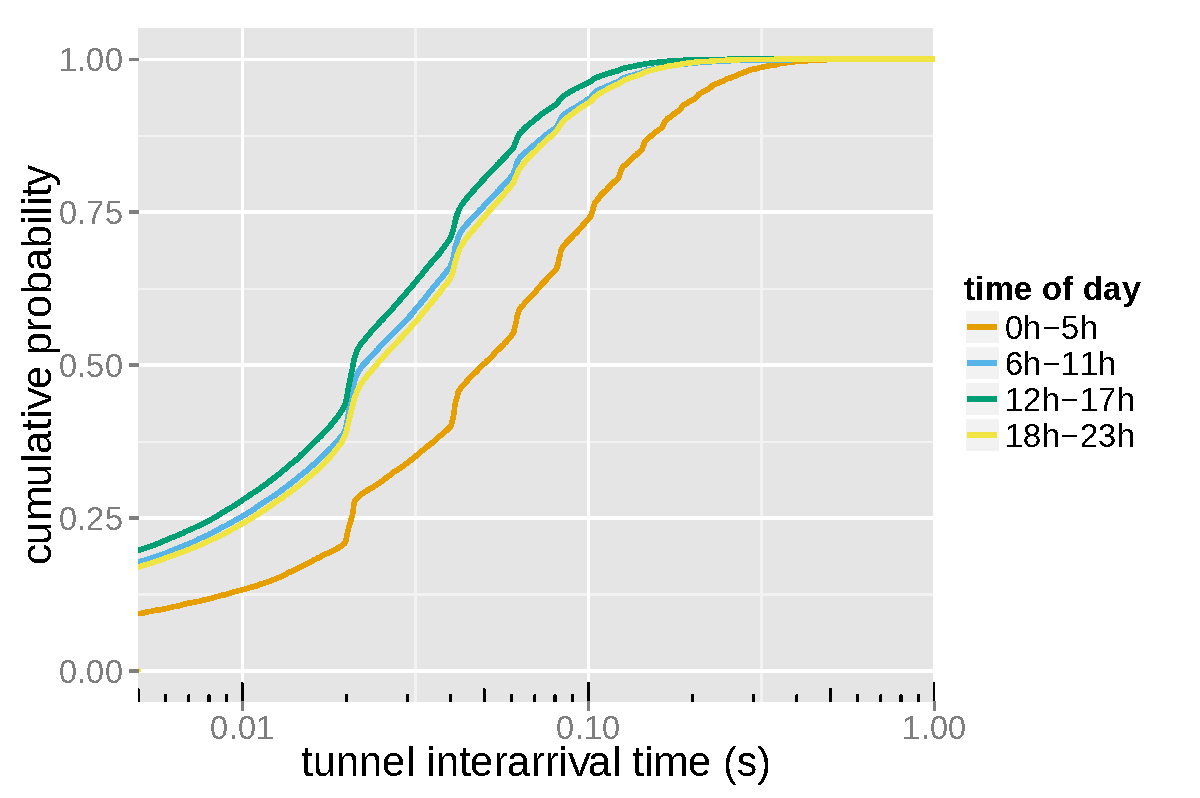
\includegraphics[width=\textwidth]{images/R-IAT-successful-2h-ecdfs.pdf}
		\caption{All tunnel requests.}
		\label{c4:fig:IAT-ecdf-2h-successful}
	\end{subfigure}%
	~
		\begin{subfigure}[b]{0.5\textwidth}
		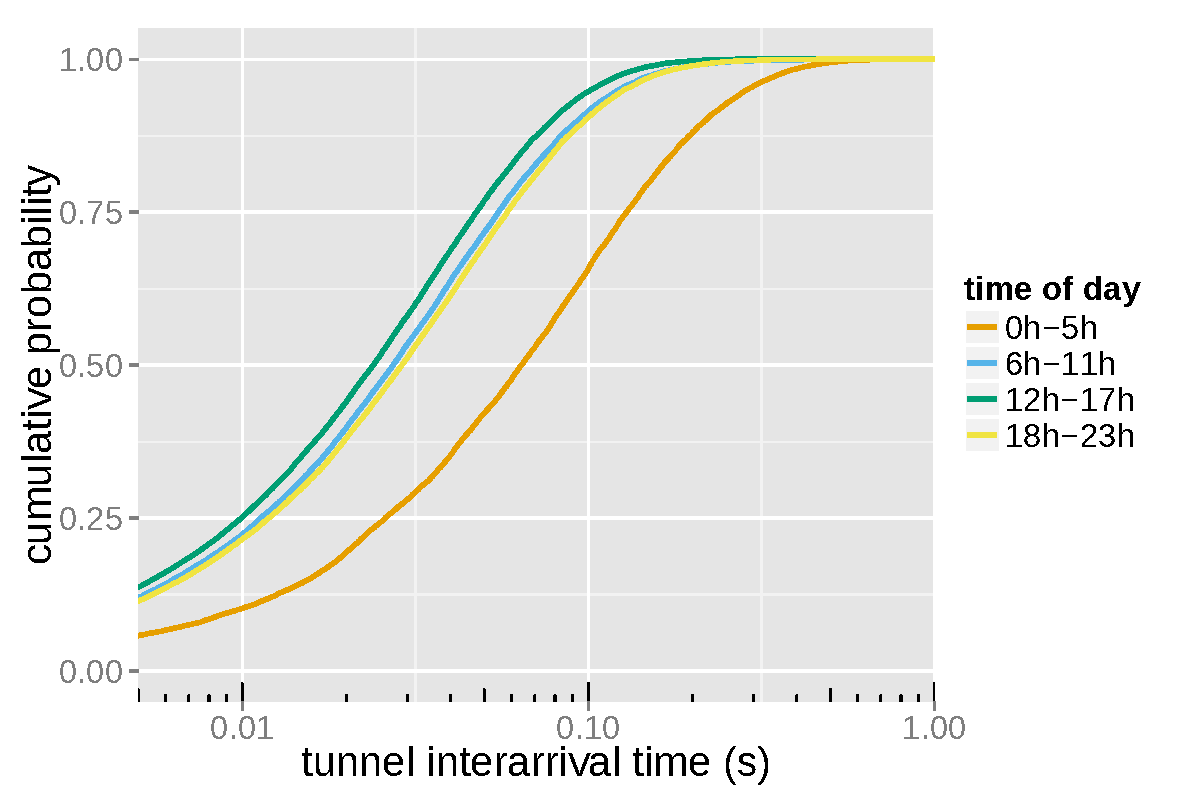
\includegraphics[width=\textwidth]{images/R-IAT-fromflows-ecdfs-2h.pdf}
		\caption{Only tunnels with data flows.}
		\label{c4:fig:IAT-ecdf-2h-active}
	\end{subfigure}

	\begin{subfigure}[b]{0.5\textwidth}
		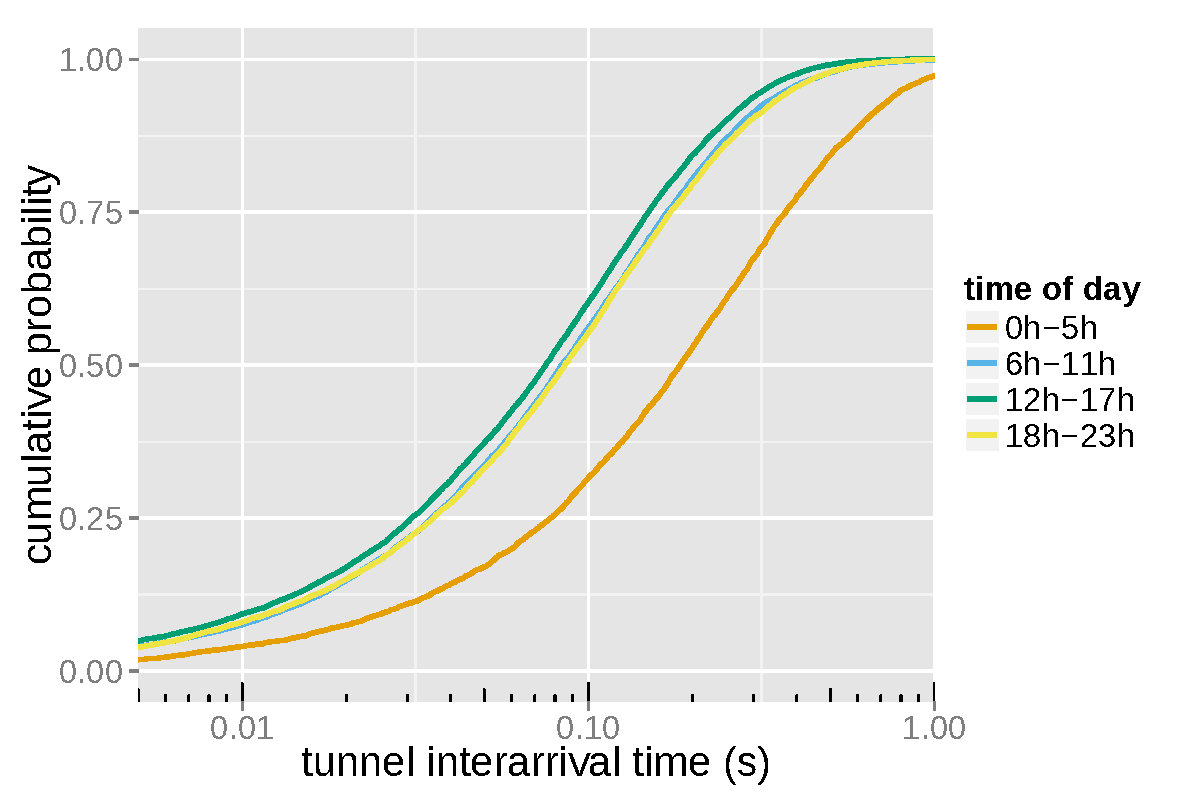
\includegraphics[width=\textwidth]{images/R-IAT-fromflows-gprs-ecdfs-2h.pdf}
		\caption{Tunnels with data flows initiated in \gls{GPRS}.}
		\label{c4:fig:IAT-ecdf-2h-active-gprs}
	\end{subfigure}%
	~
	\begin{subfigure}[b]{0.5\textwidth}
		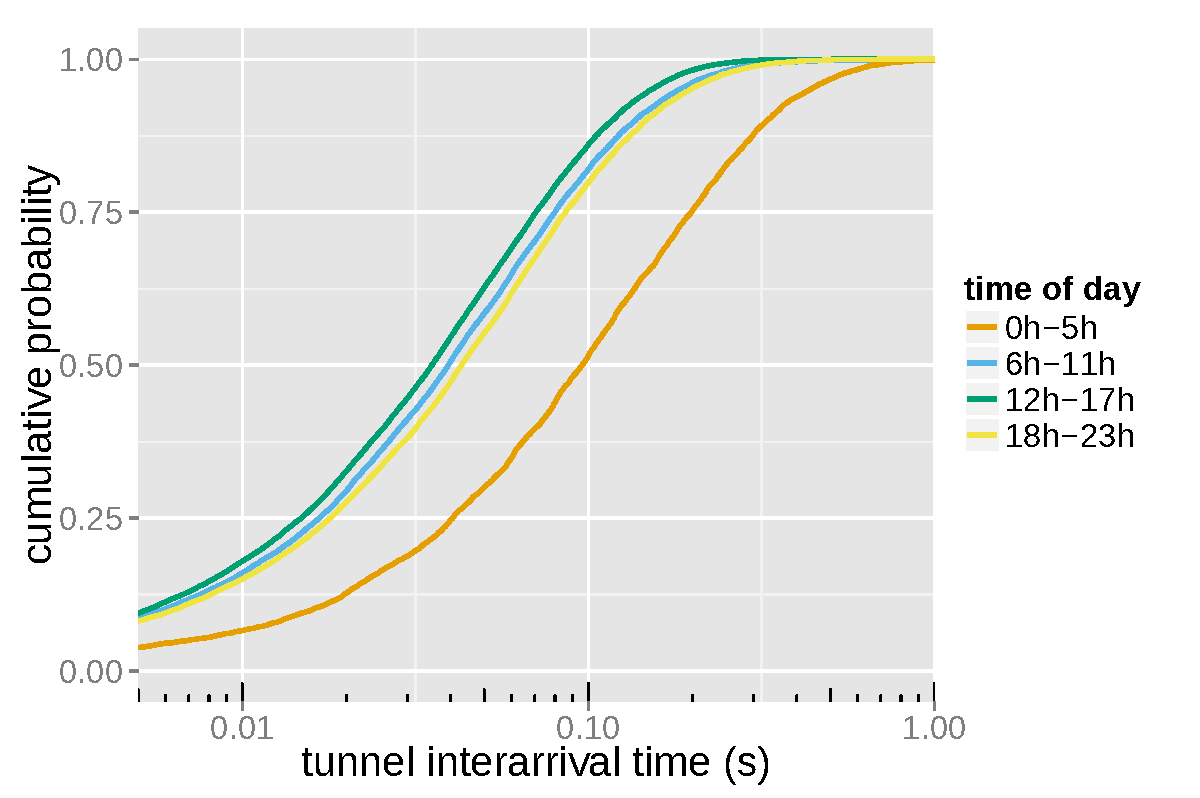
\includegraphics[width=\textwidth]{images/R-IAT-fromflows-umts-ecdfs-2h.pdf}
		\caption{Tunnels with data flows initiated in \gls{UMTS}.}
		\label{c4:fig:IAT-ecdf-2h-active-umts}
	\end{subfigure}
	\caption{\acrshortpl{ECDF} of the tunnel \acrshort{IAT} in seconds by time of day.}
\label{c4:fig:IAT-ecdf-2h}
\end{figure}

Complementing the arrival rate evaluation is the investigation of the tunnel \gls{IAT}. This metric is more sensitive to short time fluctuations of arrivals and more suited to describe the arrival process for use in the proposed load model.

The overall picture of all arrivals is given in the \gls{ECDF} of Figure~\ref{c4:fig:IAT-ecdf-2h-successful}, again broken down by time of day. Obviously the the same previously observed diurnal load oscillation can again be perceived. The median \glspl{IAT} fall in the range of \SI{20}{\milli\second} and \SI{60}{\milli\second}, enveloped by the \formattime{16}{0}{0} and \formattime{2}{0}{0}distributions on with the lowest and highest \gls{IAT} respectively. Additionally, tunnel arrivals are occurring at an increased frequency with an interval of multiples of \SI{20}{\milli\second}, which generates these wave-like steps in the \gls{ECDF} plot. As this is happening very regularly at every time of the day, a source inside the mobile network is indicated.

A hypothesis as to the origin of this effect is the value of the \gls{TTI}. This property determines the duration of a mobile network's radio transmission slot. In \gls{3GPP} standards up to \gls{UMTS} the default value of the \gls{TTI} is either \SI{10}{\milli\second} or \SI{20}{\milli\second}, newer versions of the specification set the value to \SI{2}{\milli\second} (in \gls{HSPA}) or even \SI{1}{\milli\second} (for \gls{LTE}). The absolute time of every transmission slot is also synchronized across every base station in the whole mobile network, which makes the \gls{TTI} noticeable even when not measuring directly at the radio link. 

The observed step-width of \SI{20}{\milli\second} therefore indicates, that the tunnel establishment signaling procedure includes at least one trip from the mobile device over the radio interface. This makes sense, as the tunnel is typically created during the \gls{GPRS} Attach procedure, which is indeed initiated at the user's device. Unfortunately, this gives the arrival process batch properties. As a result the load at the \gls{GGSN} increases momentarily when a batch arrives. The \gls{GGSN} would then need to process more requests simultaneously than if the arrivals followed a smooth stochastic distribution.

This effect becomes more peculiar when the tunnel arrivals are further broken down. Figure~\ref{c4:fig:IAT-ecdf-2h-active} only displays arrivals of tunnels, that actually transported user traffic during their lifetime. Here, the influence of the effect is visually unnoticeable. This could be attributed, that most active data connections during the time of the trace recording were already using almost exclusively \gls{HSPA} or better, which sees the much lower \gls{TTI}. Only older, regular phones establish plain \gls{UMTS} connections and often do not even use it.

The discrimination of the \gls{IAT} distribution by \gls{RAT} that was used during the creation of the tunnel reveals no further information. Due to the much lower number of connections the \gls{GPRS} distributions are shifted to much higher intervals than the \gls{UMTS} specific distributions.


%%%%%%%%%%%%%%%%%%%%%%%%%%%%%%%%%%%%%%%%%%%%%%%%%%%%%%%%%%%%%%%%%%%%%%%%%%%%%%%
\subsection{\texorpdfstring{\acrshort{gtp}}{GTP} Tunnel Message Processing Time}

Finally, the \gls{GGSN}'s processing time of \gls{gtp} tunnel management messages is investigated. Potentially, this can be a direct measure of the load at the node. In times of higher load one would expect a higher processing time of signaling messages.

From the network trace the processing time can be calculated by two timestamps in each record.
As the trace is recorded at the Gn interface these timestamps represent the points in time the \gls{gtp} signaling request and subsequent response pass on the link to and from the the \gls{GGSN}. Therefore, they can also be interpreted as the start and finish of the involved processing at the \gls{GGSN}.

Generally, the processing time of all three message types --- i.e., creates, deletes and updates --- could be calculated. It would be of special interest to know if the setup time of tunnels is influenced by anything, as this is one of the \gls{GGSN}'s most time-sensitive jobs and can impact the time a user has to wait before being able to actually transfer data. Unfortunately, due to unrecoverable issues with the recording of the dataset, the timestamps for both the create and delete messages records were completely unreliable and did not allow for an investigation of the processing time. 

Only \gls{gtp} update messages were unaffected and gave the opportunity for further investigation. The trace contains roughly two orders of magnitude more update messages than either creates or deletes, spread out almost evenly over the whole observation period. Therefore, a node load investigation should still be possible with just the updates messages.

\begin{figure}[htb]
	\centering
	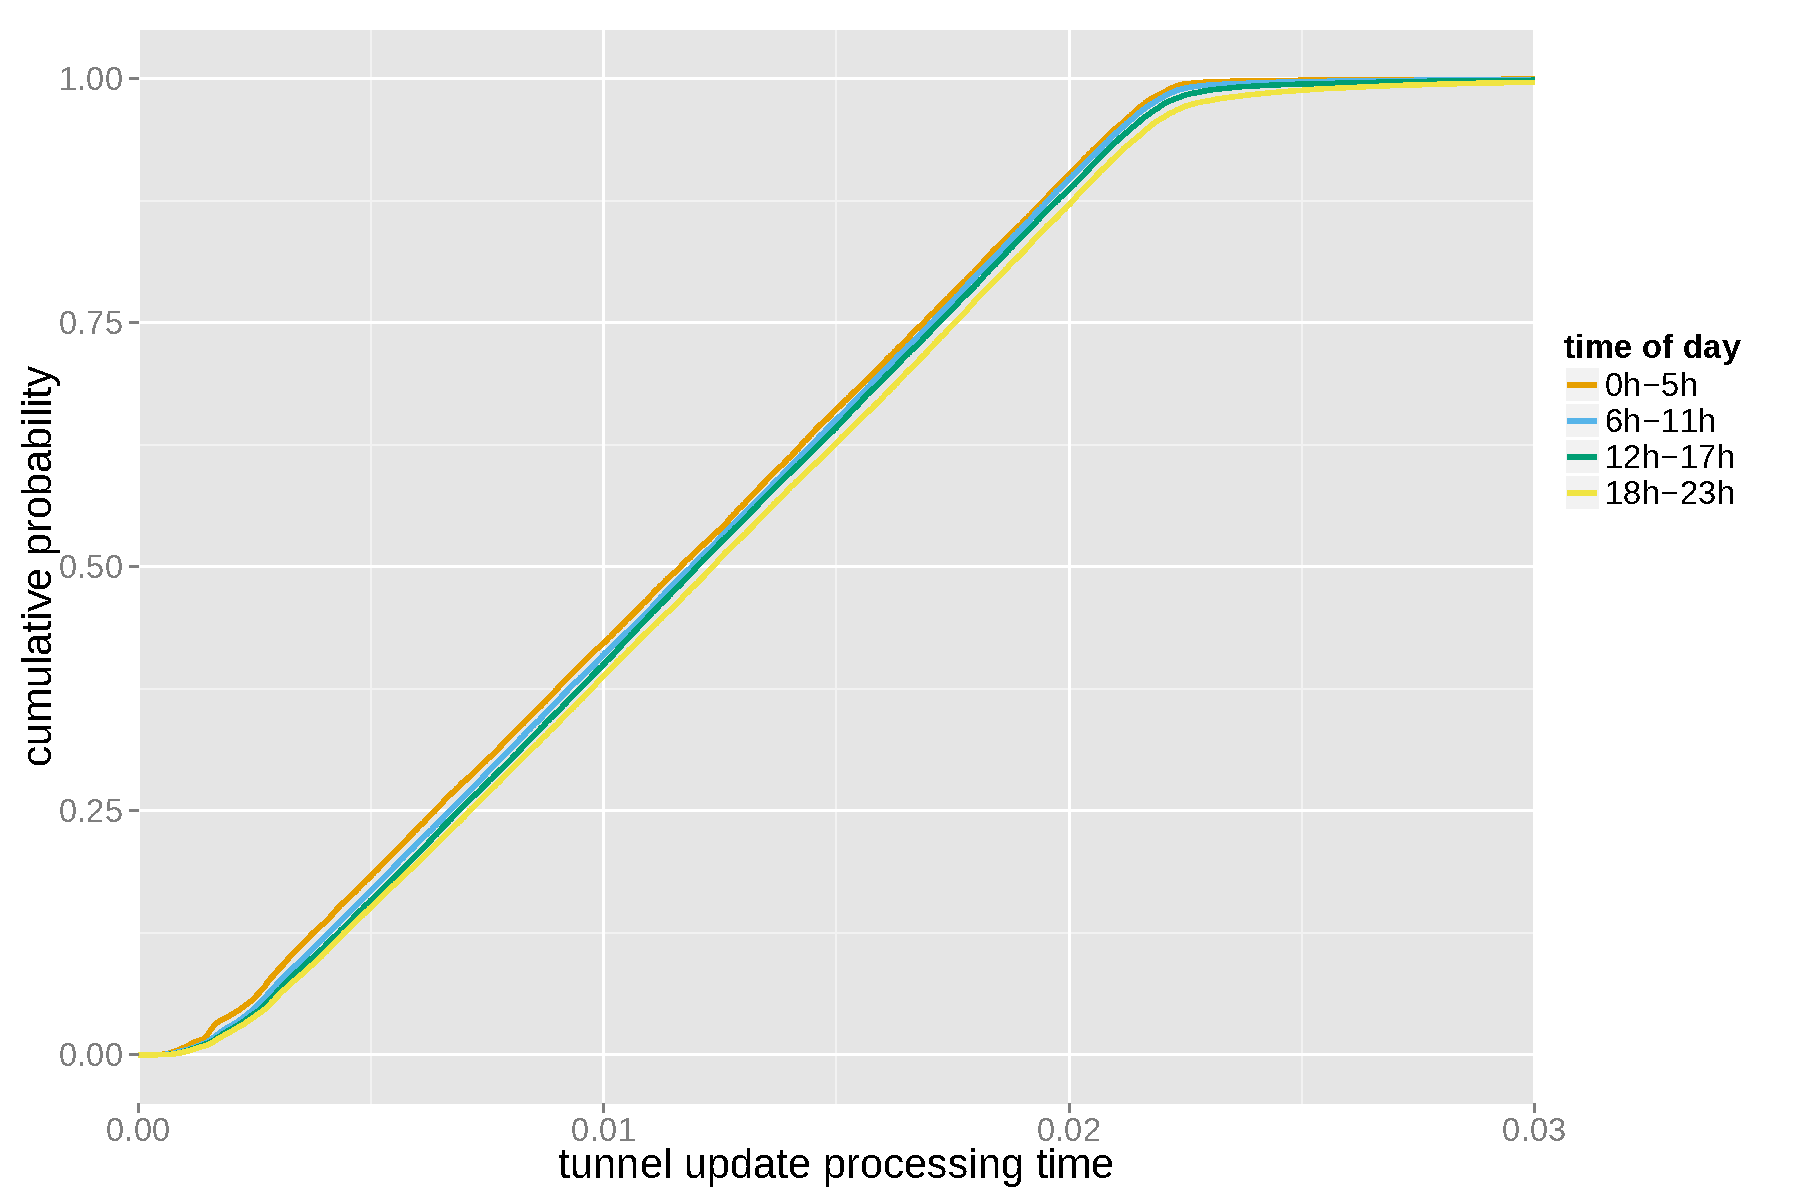
\includegraphics[width=0.9\textwidth]{images/R-update-time-cdfs.pdf}
	\caption{\acrshortpl{ECDF} of the time in seconds it takes a \acrshort{GGSN} to process a \acrshort{gtp} update event, separately plotted for four time slots each day.}
	\label{c4:fig:update-time}
\end{figure}

Figure~\ref{c4:fig:update-time} depicts a band of \glspl{ECDF} for the processing time of update messages by time of day. The processing time distribution almost perfectly follows a continuous uniform distribution between \SI{2}{\milli\second} and \SI{22}{\milli\second}. Only the upper end displays a slight long-tail behavior. The impact of the time of day is very slim with slightly higher processing times during the evening, the same time frame which also experienced an elevated arrival rate.

The occurrence of a continuous uniform distribution is rather unexpected as these do not usually occur in computing processes. According to the central limit theorem one would rather expect to see a normal distribution influenced by, e.g., process scheduling or other queuing artifacts. The source of this effect is still unknown and the current dataset does not allow for a more thorough investigation. Still, the fact that a higher update processing time coincides with an increase in the arrival rate points to an influence of tunnel messaging on the load of a \gls{GGSN}.



%%%%%%%%%%%%%%%%%%%%%%%%%%%%%%%%%%%%%%%%%%%%%%%%%%%%%%%%%%%%%%%%%%%%%%%%%%%%%%%
\subsection{Statistical Evaluation and Data Fitting}
\label{c4:sec:statistical_evaluation}

The uncovered empirical distributions for both the tunnel duration and the tunnel \gls{IAT} are now to be matched against theoretical probability distributions. Therefore, a univariate distribution fit to the experimental data was conducted. Having a concise representation for the empirical data will help in creating a model of the core network, which is the task conducted in the sections following after this.


%%
\paragraph{\gls{IAT} Fitting}

\begin{figure}[htb]
	\centering
	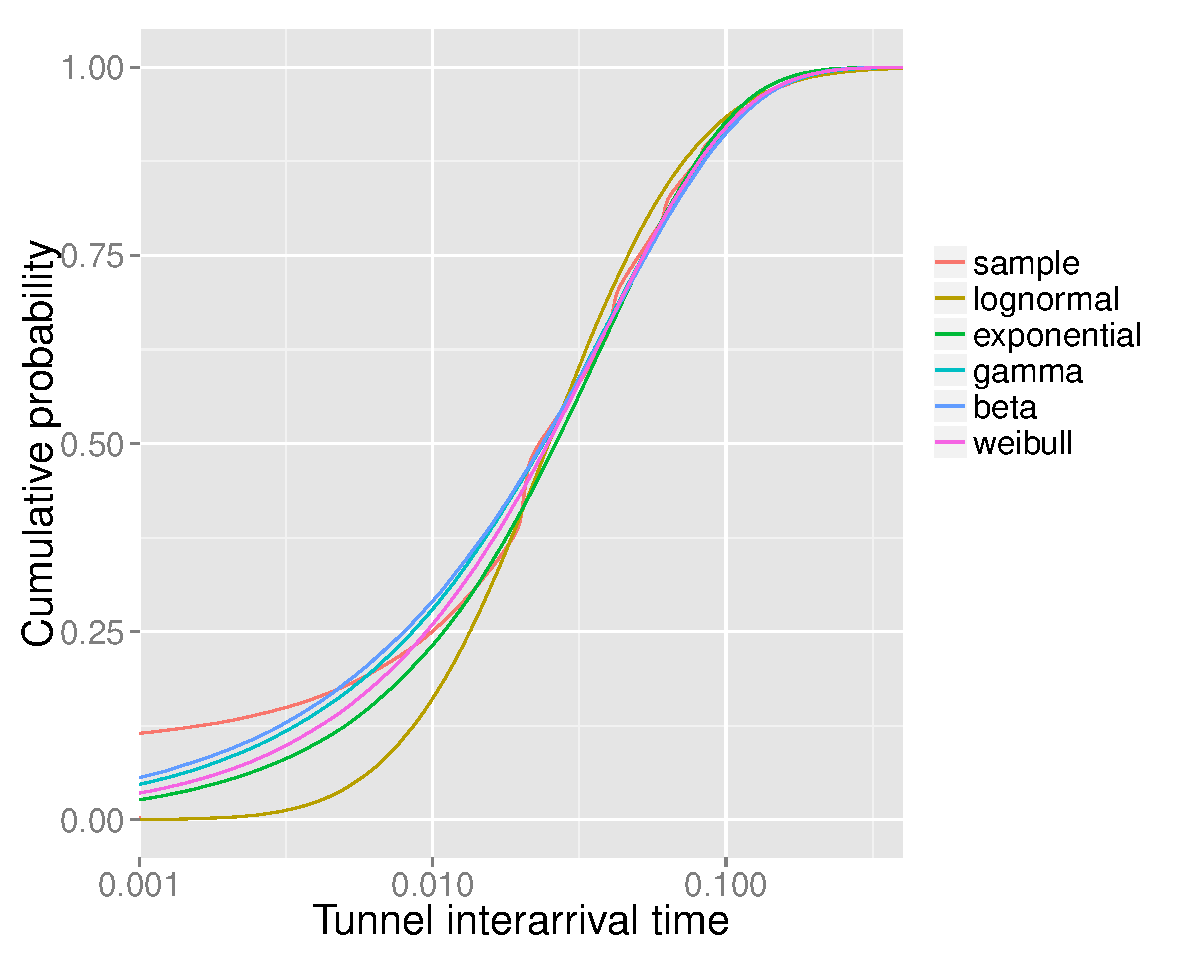
\includegraphics[width=0.9\textwidth]{images/R-IAT-ecdfs.pdf}
	\caption{Sampled inter-arrival time \acrshort{CDF} and fitted theoretical distributions.}
\label{c4:fig:IAT-cdfs}
\end{figure}

In order to investigate the tunnel \gls{IAT}, Figure~\ref{c4:fig:IAT-cdfs} displays the overall \gls{ECDF} with fits for various basic probability distributions. Each of the fits was generated through the method of moments matching.

The goodness of these fits was checked both visually using the \glspl{CDF} plots and numerically with goodness of fit measures, using Pearson's correlation coefficient and Pearson's $\chi^2$ test. Unfortunately, none of the probability distributions reaches the significance level for $\chi^2$. This can probably be largely attributed to the various previously described artifacts in the data. Matching them visually, the exponential fit seems to be reasonably close to the experimental data.

\begin{figure}[htb]
	\centering
	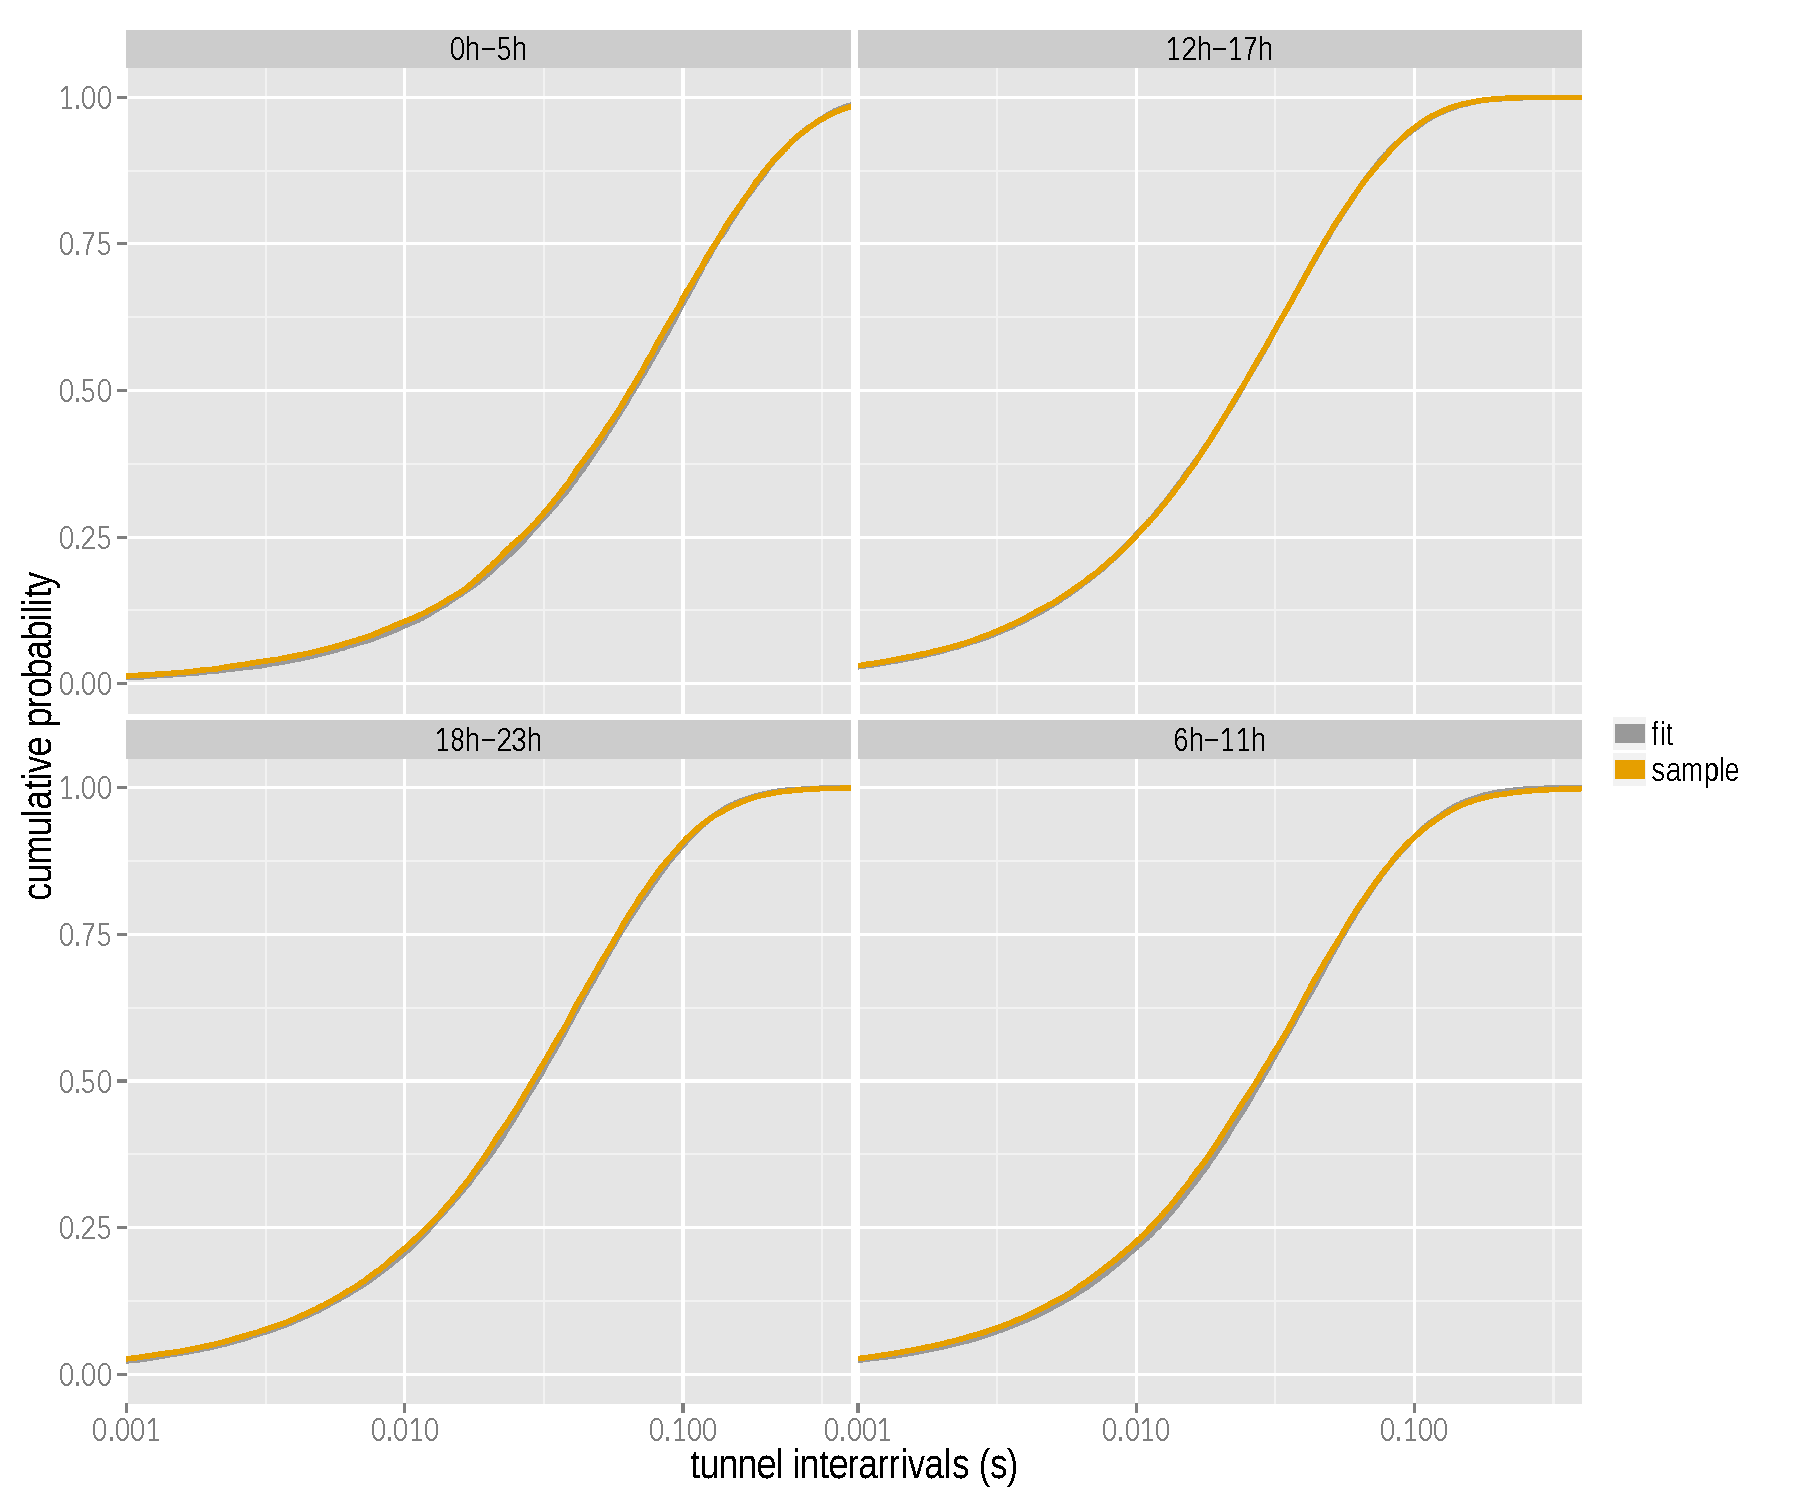
\includegraphics[width=0.9\textwidth]{images/R-IAT-active-fit-cdf-facets.pdf}
	\caption{Empirical and exponentially fitted \acrshortpl{CDF} of the tunnel \acrshort{IAT} by time of day. \acrshortpl{CDF} are overlapping as the coefficient of determination is close to $1$.}
\label{c4:fig:pdparrivalsecdf}
\end{figure}

To improve the fits, two modifications were made to the process. First, to remove the \SI{20}{\milli\second} steps, only the active tunnels were taken into consideration. Second, the overall \gls{IAT} distribution was once again split up into time of day slots. The overall distribution is just a superimposition of the individual slots anyway. Therefore, this should further improve the fidelity of the fits.

\begin{table}[htb]
\caption{Parameters for the exponentially distributed inter-arrival times and corresponding Pearson correlation coefficients.}
\label{c4:tab:IAT-fits}
	\centering
	\begin{tabu}{X[0.9,l]X[r]X[r]} 
	\toprule
	\textbf{Time of Day} & $\mathbf{\lambda}$ & $\mathbf{R_{arrival}}$\\ 
	\midrule
	0h-5h   & $10.67477$ & $0.995$ \\
	6h-11h  & $24.53298$ & $0.992$ \\
	12h-17h & $29.2504$  & $0.993$ \\
	18h-23h & $23.49983$ & $0.986$ \\
	\bottomrule
	\end{tabu}
\end{table}

The results are depicted in Figure~\ref{c4:fig:pdparrivalsecdf}. To improve plot visibility only four larger time slots are displayed here while the actual fits were conducted for each hour slot. Parameters for the exponential distribution $F(x) = 1- e^{-\lambda x}, x \geq 0$ and the corresponding correlation coefficients to the original data for the four time slots are given in Table~\ref{c4:tab:IAT-fits}. The fitted functions match the empirical data quite well, with some deviation present at the left tail but an overall positive correlation coefficient approaching $1$.


%%
\paragraph{Duration Fitting}

The second fitting effort surrounds the empirical data concerning the tunnel durations. However, none of the basic probability distributions (including exponential, gamma, and Weibull distributions) fit the tunnel duration even remotely. One of the reasons for this is probably, that the tunnel duration is influenced by an overwhelming amount of factors, which were previously described. This superposition, especially with the user behavior, will result in unpredictable results that does not follow any basic probability distribution.

\begin{figure}[htb]
	\centering
	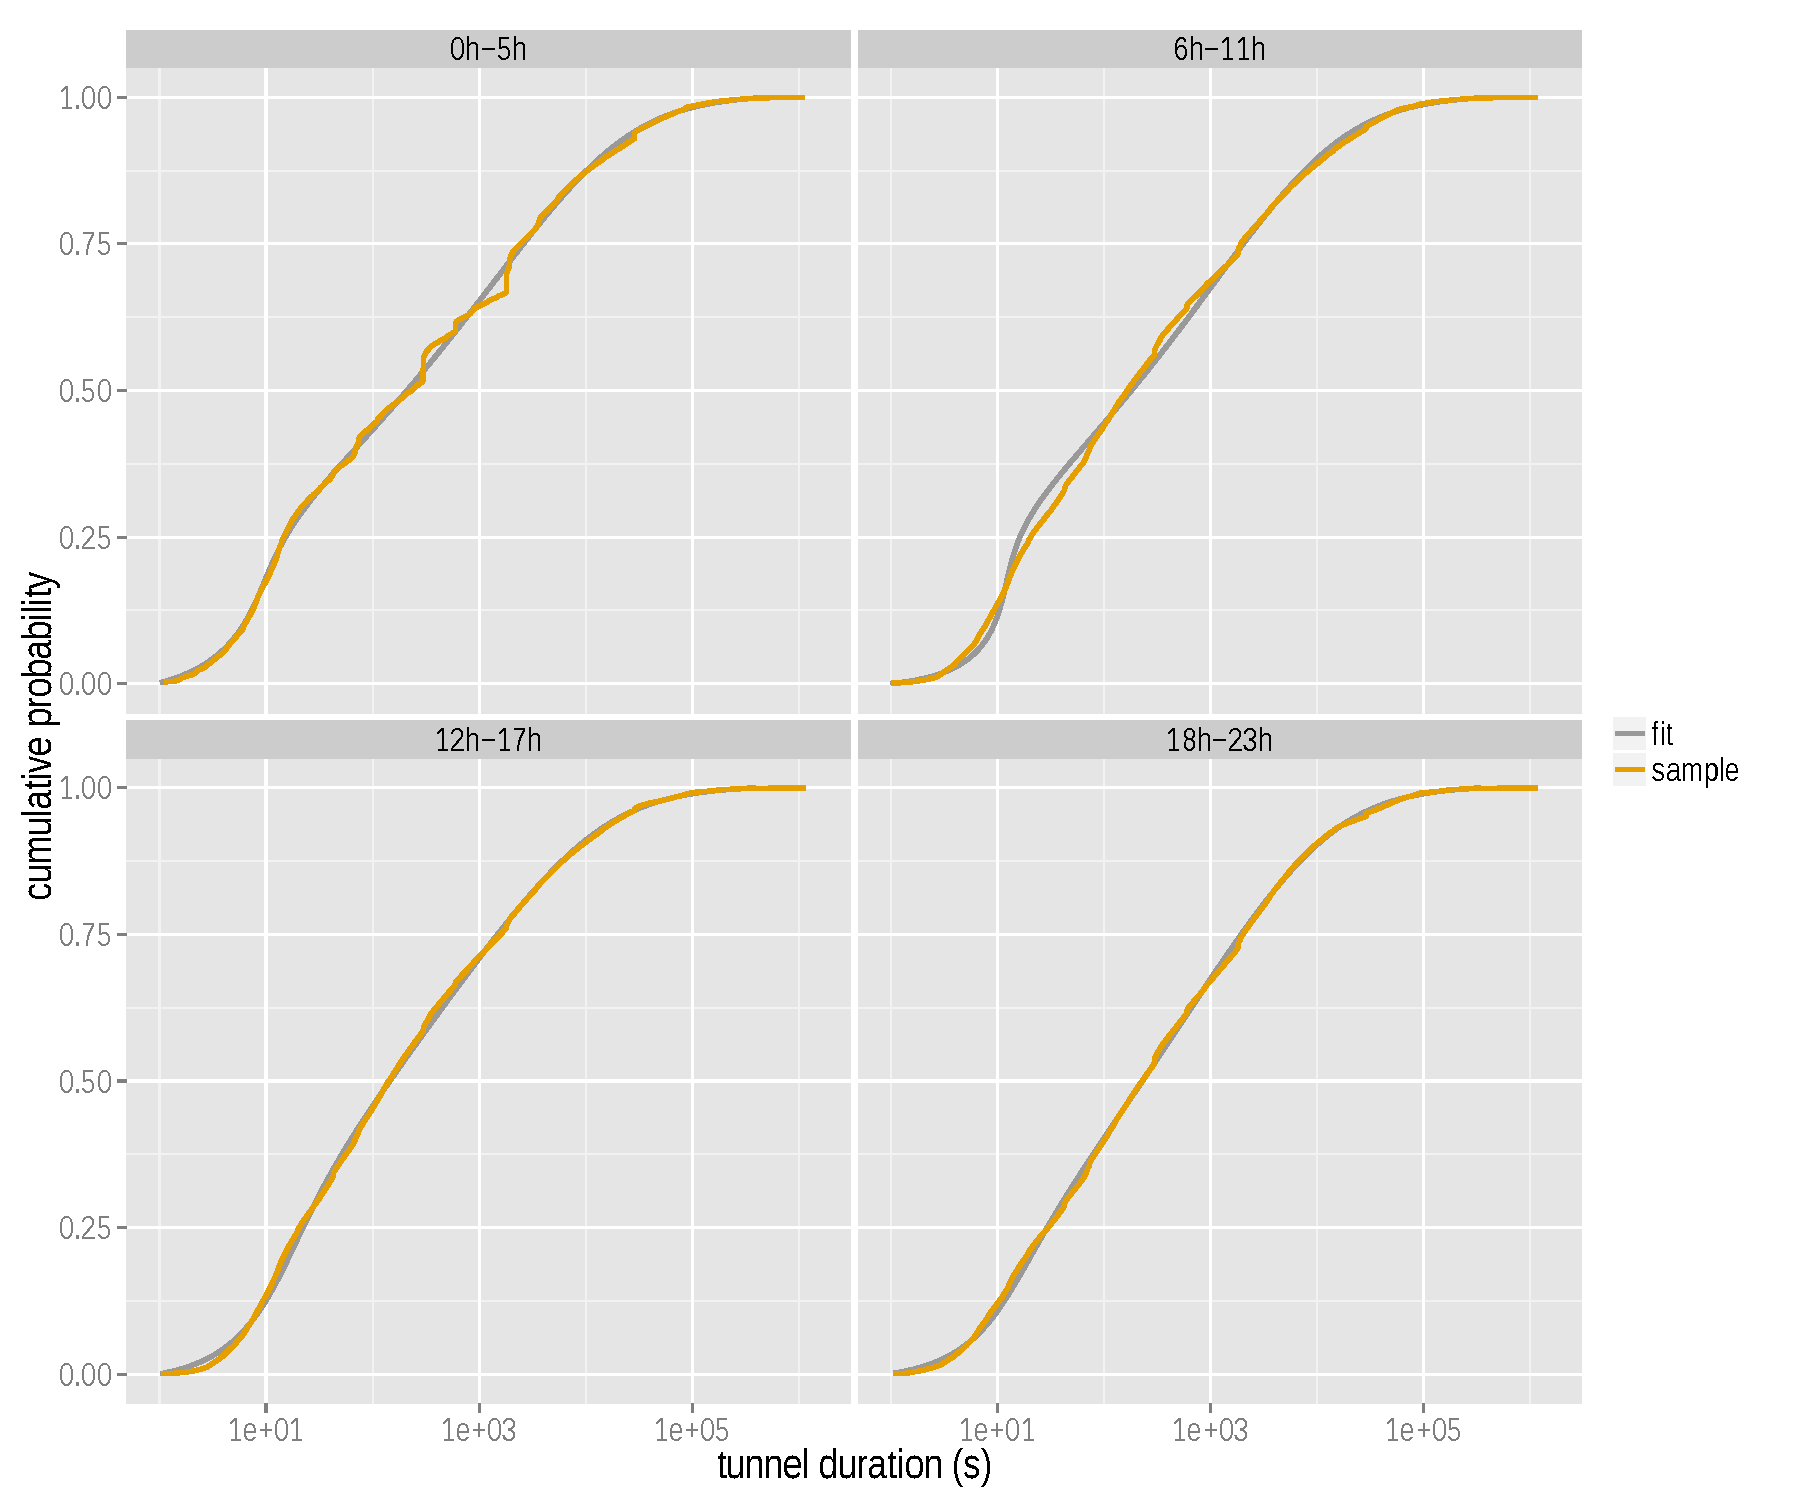
\includegraphics[width=0.9\textwidth]{images/R-duration-fit-cdf-facets.pdf}
	\caption{Empirical and fitted \acrshortpl{CDF} of the tunnel duration by time of day with fitted rational functions.}
\label{c4:fig:fittedsdurationlots}
\end{figure}

Instead, rational functions are fitted to the \glspl{ECDF} using the proprietary third-party tool \textit{Eureqa}~\cite{eureqa_paper, eureqa_software}. This allows for a much closer fit as seen in Figure~\ref{c4:fig:fittedsdurationlots}, but limits its application in the statistical evaluation.

\begin{table}[htb]
\caption{Inverse rational functions fitted to the \acrshortpl{ECDF} of the tunnel duration by time of day and correlation coefficients of the fit.}
\label{c4:tab:fits-duration}
	\centering
	\begin{tabu}{X[1.1,l]X[4.5,r]X[r]} 
	\toprule
	\textbf{Time of Day} & \textbf{Inverse Serving Time \gls{CDF} Representation} & $\mathbf{R_{dur}}$\\ 
	\midrule
	0h-5h & $0.919208 - 60.6136y - 3498.78y^3 - \frac{110.707y + 2289.94y^3}{y - 1.00469}$ &  $0.999$ \\
	6h-11h & $1 + 117.484y - 368.643y^2 - \frac{1720.13y^4}{y - 1.0041}$ & $0.999$ \\
	12h-17h & $0.952566 + 69.4907y + \frac{81146.1y^3 + 1.08572\times10^6y^5}{805 - 802.01y}$ & $0.999$ \\
	18h-23h & $0.911924 + 82.0562y - \frac{2936.93y^4}{1.94468y - 1.9532}$ & $0.999$ \\
	\bottomrule
	\end{tabu}
\end{table}

Table~\ref{c4:tab:fits-duration} contains the functions which were fitted to the \textit{inverse} \gls{CDF}. The inverse was chosen here to simplify the modeling and simulation process coming afterwards. The functions can be easily inverted again for other purposes. Both the \glspl{CDF} in the plot as well as the Pearson correlation coefficient, which again approach $1$, confirm the goodness of the fitted functions.


% \begin{table}
% \centering
% \caption{TAC Statistics}
% \begin{tabu}{|X|X|X[1.5]|X|X|X|} \hline
% & \textbf{\# of Flows} & \textbf{Total Traffic (Bytes)} &  \textbf{\# of Tunnels} & \textbf{\# of GTP Signalling Msgs} & \textbf{\# of Distinct IMSIs}\\ \hline
% Total          & 2234659247 & 122758578593993 (112TB)    & 16632094 & 409733865 & 1255293 (all) / 1030895 (with flows) \\ \hline
% In TAC DB      & 2228315260 & 122716712007150 (111.61TB) & 14565430 & 372662108 & 1015891 \\ \hline
% Smartphones    & 459990512  & 15721818747754 (14.30TB)   & 10030734 & 311342846 & 476675  \\ \hline
% Regular phones & 5705832    & 448140315058 (0.41TB)      & 897529   & 3860162   & 116124  \\ \hline
% 3G dongles     & 1487230062 & 92215931895630 (83.87TB)   & 2114756  & 39053819  & 315003  \\ \hline
% Android        & 241973565  & 7953178401958 (7.2TB)      & 2383255  & 177537567 & 175919  \\ \hline
% iOS            & 161408903  & 5481693567152 (5TB)        & 3145384  & 83374590  & 99679   \\ \hline
% Symbian        & 22827418   & 1332996529271 (1.21TB)     & 3520242  & 18479002  & 162790  \\ \hline
% Blackberry OS  &            & 128074907884 (0.12TB)      &          &           &         \\ \hline
% \end{tabu}
% \end{table}


%Devices with GTP signaling but no user plane traffic: (\#distinct imsis gtp db)-(\#distinct imsis flow db):
% $255293-1030895=224398\text{ or }17.88\%$

%%%%%%%%%%%%%%%%%%%%%%%%%%%%%%%%%%%%%%%%%%%%%%%%%%%%%%%%%%%%%%%%%%%%%%%%%%%%%%%%
%\subsection{Correlations to User Traffic}
% TODO, incl. measurements



%%%
% Direct signaling traffic overhead in relation to user traffic and induced network load

% GTP Header: 12 Byte
% IE header and footer: 2 Byte
% Maximum minimum data size including all \glspl{IE}: 221 Byte + 12 Byte Header + 2*37 Extension Header = 307 Byte
% Minimum size of message with just mandatory \glspl{IE}: 12 + 30 + 2*5 = 52 Byte

% 307 Bytes:
% calculation from our dataset
% Total maximum signaling traffic with this calculation: 117.15GB
% Ratio: 0.10\%
% 52 Bytes:
% Total maximum signaling traffic with this calculation: 19.84GB
% Ratio: 0.02\%
% Total traffic: 122758578593993


% signaling calc:
% gtp signaling traffic volume estimation $v_s$ = (1059B gtp message + 8B udp header + 20B ipv4 header) = 1087B * 409733865 number of request/response pairs * 2 (2 messages per pair) = 8,9076142E11B
% ratio to total $r=\frac{v_s}{v_t}=0.72\%$  $v_t=122758578593993B$


%%
%TODO: radio access type plots, if we have the data
% We do not.
%
%\begin{figure}
%\centering
%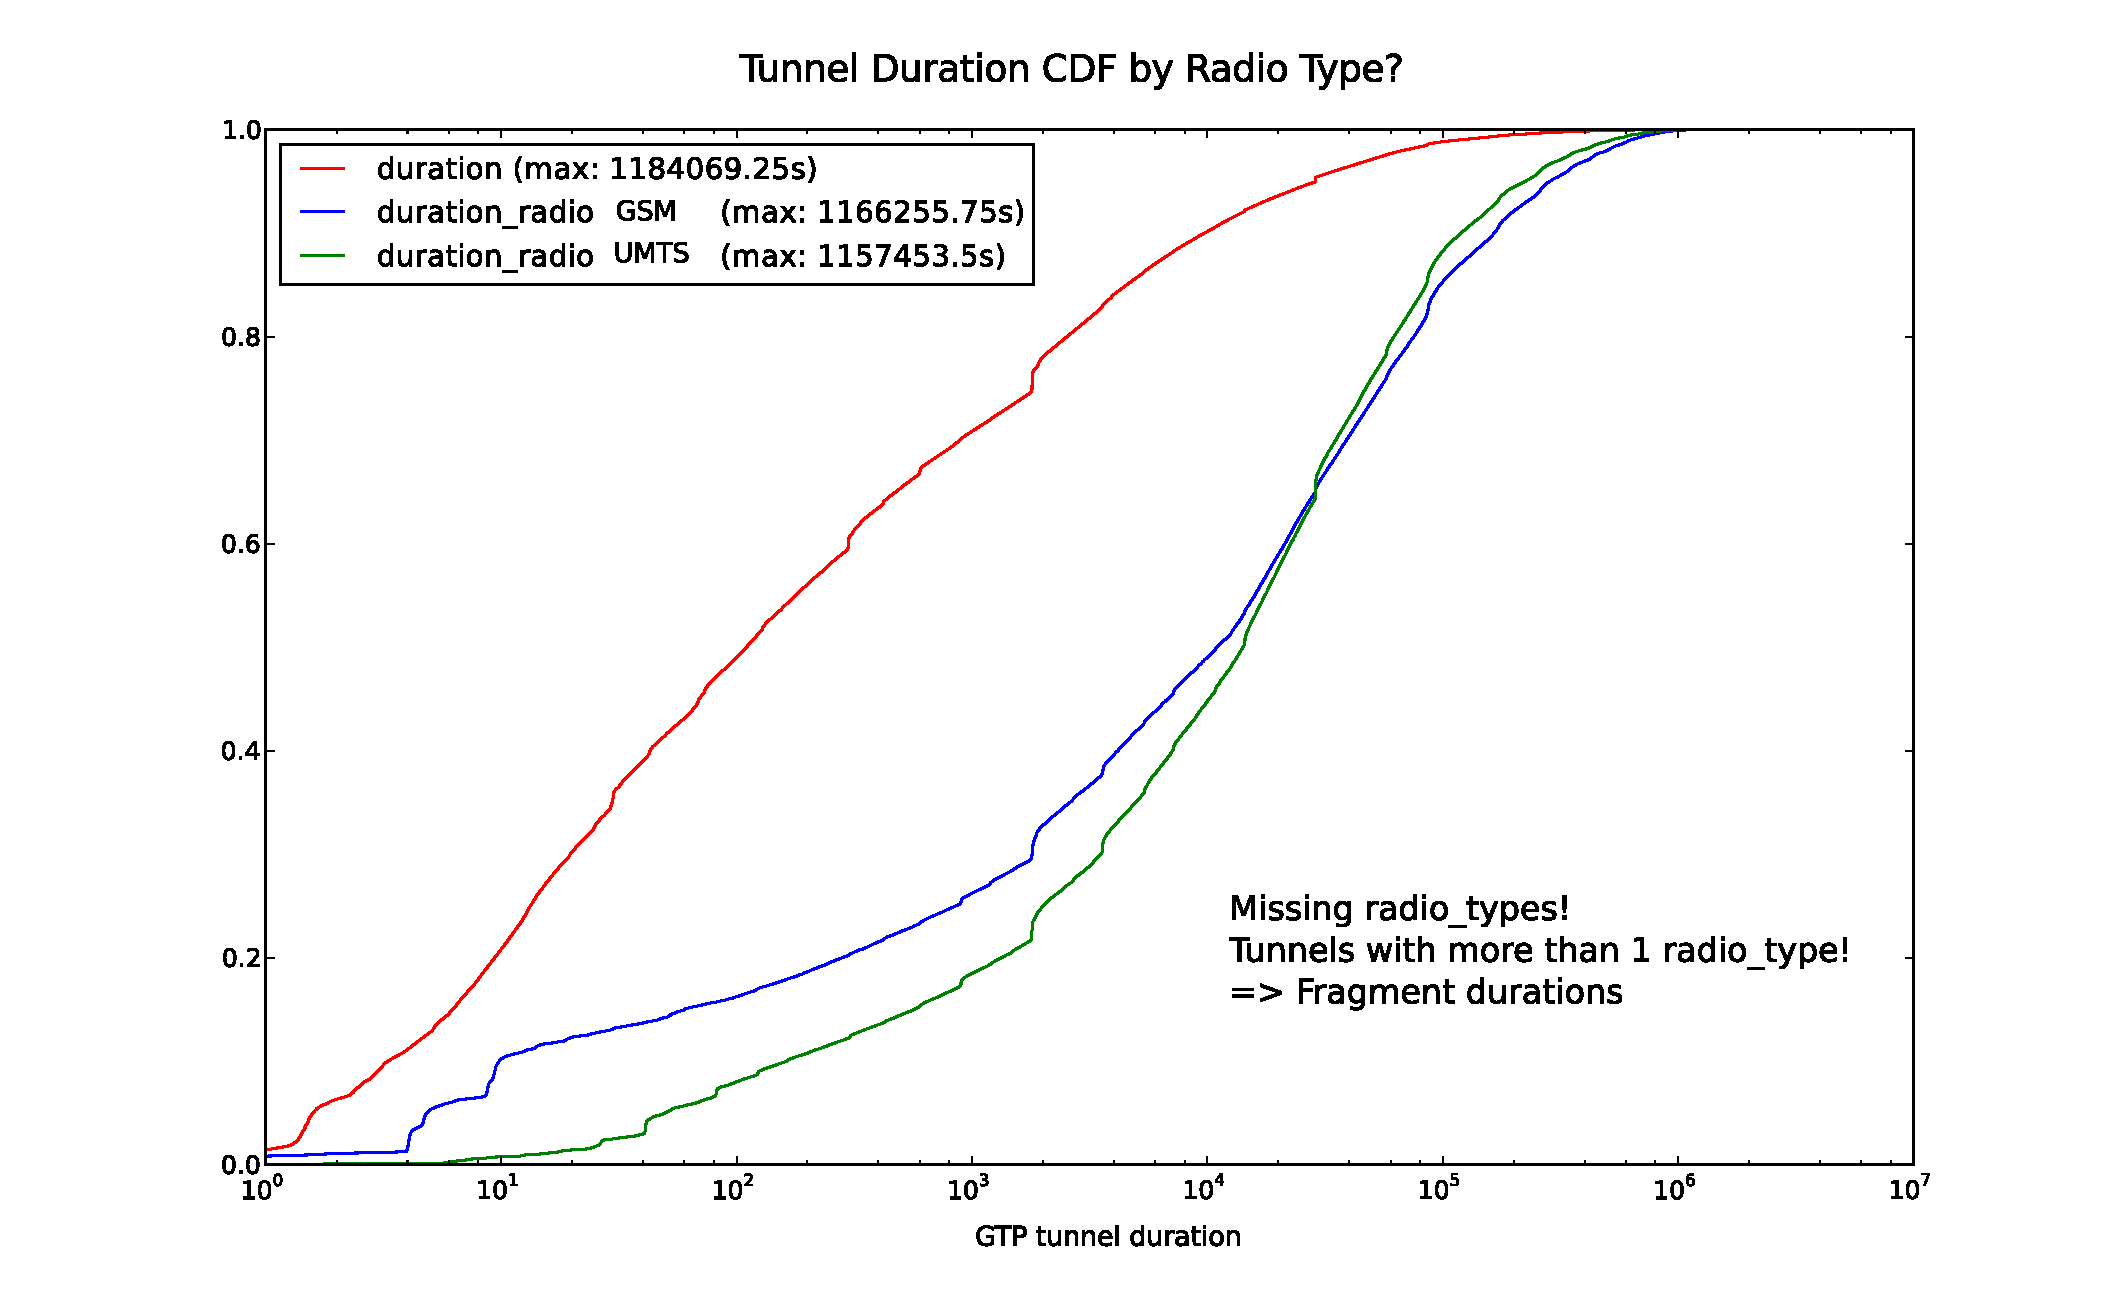
\includegraphics[width=\columnwidth]{figures/tunnel-dur-radio-cdf-mod.pdf}
%\caption{Tunnel duration distribution, separated for UMTS and GPRS radio access [NOTE: only in the last tunnel segment; and majority of radio types %is unknown anyway.}
%\label{fig:cdf-duration-radio}
%\end{figure}